% \documentclass{article}
% \input{../preamble}
% \usepackage{scalerel}
% \input{unit10glossary}

% \usepackage{fancyhdr}
% \pagestyle{fancy}
% \renewcommand{\headrulewidth}{0pt}
% \renewcommand{\headruleskip}{0mm}
% \fancyhead{}

% \numberwithin{equation}{section}
% \setcounter{section}{10}
% \numberwithin{figure}{section}


% \title{Unit 11: Waves}
% \author{Physics\footnote{Access for free at \href{\openstax}{\openstax}} \hspace{0.1ex} at Cypress Springs High School}
% \date{Updated on \today}
% \openstaxfooter

% \makenoidxglossaries

\documentclass[main.tex]{subfiles}

\begin{document}

\section{waves}


\subsection{Introduction} \label{R3JSIu}

A \gls{wave} is a disturbance that moves from a source and carries energy. Light, sound, and ocean waves are common examples of waves. Waves \gls{propagate}, or move in a given direction. A \gls{mechanical wave} is a wave that requires a medium through which it can travel. The \gls{medium} is the solid, liquid, or gas material through which a wave propagates. 

\vspace{1em}

A \gls{transverse wave} is a wave in which the disturbance is \textit{perpendicular} to the direction of propagation. 


\begin{center}
    \centering
    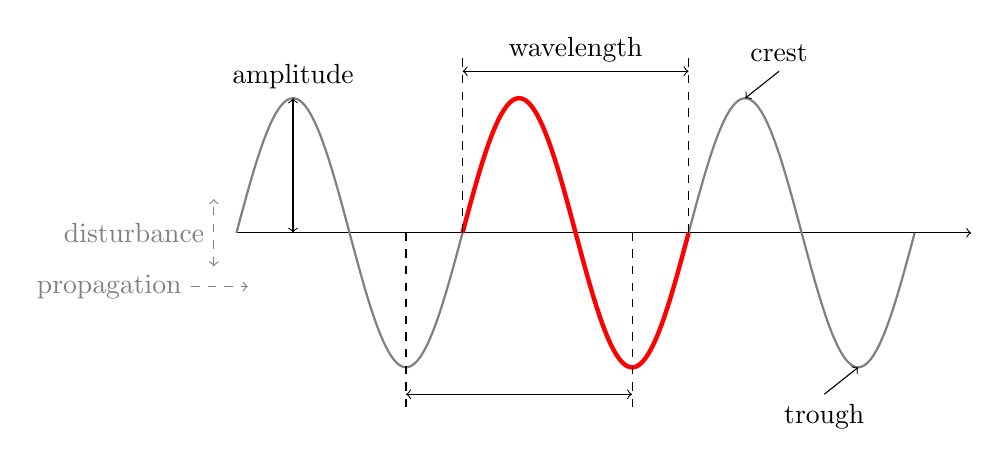
\begin{tikzpicture}
\begin{axis}[width=0.9\textwidth,height=5cm,
    xmin=0,xmax=6.5,
    ymin=-1,ymax=1,
    clip=false,
    ticks=none,
    axis line style={draw=none}]
    \draw[->] (0,0) -- ++ (axis direction cs: 6.5,0);
    \draw[thick, gray] plot[domain=0:6*pi, samples=200]  (\x/pi,{sin(\x r)});
    \draw[ultra thick,red] plot[domain=2*pi:4*pi,samples=100]   (\x/pi,{sin(\x r)});
    \draw[<->] (0.5,0) -- ++(axis direction cs: 0,1) node[above] {amplitude};
    \draw[<-] (4.5,1) -- ++(axis direction cs: 0.3,0.2) node[above] {crest};
    \draw[<-] (5.5,-1) -- ++(axis direction cs: -0.3,-0.2) node[below] {trough}; 
    \draw[dashed] (2,0) -- ++(axis direction cs: 0,1.3) (4,0) -- ++(axis direction cs: 0,1.3);
    \draw[<->] (2,1.2) -- ++(axis direction cs: 2,0) node[above,pos=0.5] {wavelength};
    \draw[dashed] (1.5,0) -- ++(axis direction cs: 0,-1.3) (3.5,0) -- ++(axis direction cs: 0,-1.3);
    \draw[<->] (1.5,-1.2) -- ++(axis direction cs: 2,0);
    \draw[gray,dashed,<->] (-0.2,-0.25) -- ++(axis direction cs: 0,0.5) node[left,pos=0.5] {disturbance};
    \draw[gray,dashed,->] (-0.4,-0.4) node[left] {propagation} -- ++(axis direction cs: 0.5,0);
\end{axis}
\end{tikzpicture}
    \captionsetup{type=figure,margin=1in}
    \captionof{figure}{A transverse wave and its different parts.}
    \label{UsT9n9}
\end{center}

There are several parts of a transverse wave. First we note that waves \gls{oscillate}, which means they move back and forth regularly between two points. The \gls{crest} is the highest position in the cycle of a wave. Likewise, the \gls{trough} is the lowest position in the cycle of a wave. The \gls{amplitude} is the maximum displacement from the equilibrium position of a wave's segment oscillating around the equilibrium position. Amplitude is related to the wave's energy. You can think amplitude as the ``height'' of a crest. \Gls{wavelength} is the horizontal distance between \gls{adjacent}\footnote{Adjacent means ``next to''} identical parts of a wave. For convenience, you can measure wavelength as the distance between two adjacent crests. The distance between two adjacent troughs is also a wavelength. 

\subsection*{\ref{R3JSIu} Exercises}

\begin{exercise}
    Watch ``Wave Machine Demonstration'' by \texttt{National STEM Centre} on \texttt{YouTube} (\href{https://youtu.be/VE520z_ugcU}{click here}).
\end{exercise}

\begin{exercise}
    Access the ``Wave on a String'' \texttt[red]{PhET Simulation} (\href{https://phet.colorado.edu/en/simulation/wave-on-a-string}{click here}). Press the play button to start the simulation, then press the \texttt[red]{No End} option. As you move the pipe wrench vertically up and down, observe the direction in which the wave propagates. Draw a sketch of this simulation, and use your sketch to explain the definition of a \gls{transverse wave}.
\end{exercise}

\begin{exercise}
    Write the definitions of each of the following words: wave, propagate, mechanical wave, medium, transverse wave, oscillate, crest, trough, amplitude, wavelength, adjacent, wave cycle, and wave velocity. If helpful, draw a sketch to accompany your definitions.
\end{exercise}

\cyanhrule


\subsection{Wave Cycles}\label{ZAl8Xb}

A \gls{wave cycle} is any portion of a wave encompassed by 1 wavelength. Figure \ref{P6fpGJ} below shows four unique examples of a single wave cycle, each of which is highlighted in red.

\begin{center}
    \centering
    \def\xmax{12}
    \begin{tikzpicture}
\begin{axis}[width=0.9\textwidth,height=3.5cm,
    xmin=0,xmax=\xmax,
    ymin=-1,ymax=1,
    clip=false,
    ticks=none,
    axis line style={draw=none}]
    \draw[lightgray] (0,0) -- ++ (axis direction cs: \xmax,0);
    \draw[lightgray] plot[domain=0:\xmax*pi, samples=200]  (\x/pi,{sin(\x r)});
    \draw[ultra thick,red] plot[domain=0*pi:2*pi,samples=100]   (\x/pi,{sin(\x r)});
    \draw[dashed] (0,0) -- ++(axis direction cs: 0,1.3) (2,0) -- ++(axis direction cs: 0,1.3);
    \draw[<->] (0,1.2) -- ++(axis direction cs: 2,0) node[above,pos=0.5] {1 wave cycle};
    %%% 
    \draw[ultra thick,red] plot[domain=3.5*pi:5.5*pi,samples=100]   (\x/pi,{sin(\x r)});
    \draw[dashed] (3.5,0) -- ++(axis direction cs: 0,-1.3) (5.5,0) -- ++(axis direction cs: 0,-1.3);
    \draw[<->] (3.5,-1.2) -- ++(axis direction cs: 2,0);% node[above,pos=0.5] {1 wave cycle};
    %%%
    \draw[ultra thick,red] plot[domain=6.5*pi:8.5*pi,samples=100]   (\x/pi,{sin(\x r)});
    \draw[dashed] (6.5,0) -- ++(axis direction cs: 0,1.3) (8.5,0) -- ++(axis direction cs: 0,1.3);
    \draw[<->] (6.5,1.2) -- ++(axis direction cs: 2,0);% node[above,pos=0.5] {1 wave cycle};
    %%%
    \draw[ultra thick,red] plot[domain=9.25*pi:11.25*pi,samples=100]   (\x/pi,{sin(\x r)});
    \draw[dashed] (9.25,0) -- ++(axis direction cs: 0,-1.3) (11.25,0) -- ++(axis direction cs: 0,-1.3);
    \draw[<->] (9.25,-1.2) -- ++(axis direction cs: 2,0);%
\end{axis}
\end{tikzpicture}
    \captionsetup{type=figure,margin=1in}
    \captionof{figure}{Four examples of one wave cycle.}
    \label{P6fpGJ}
\end{center}

\begin{example}
    How many wave cycles are shown in the wave below?
\end{example}

\begin{center}
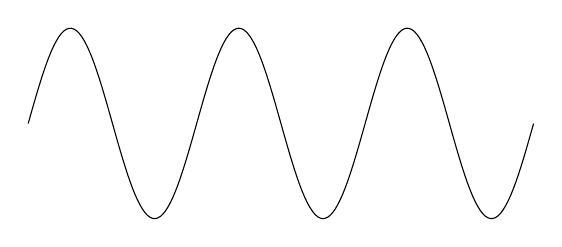
\begin{tikzpicture}
\begin{axis}[width=8cm,height=4cm,
    xmin=0,xmax=6,
    ymin=-1,ymax=1,
    clip=false,
    ticks=none,
    axis line style={draw=none}]
    \draw plot[domain=0:6*pi, samples=200] (\x/pi,{sin(\x r)});
\end{axis}
\end{tikzpicture}
\end{center}


\Solution There are exactly 3 wave cycles. In the figure below, the first wave cycle in highlighted in red. The end points of the subsequent wave cycles are labeled as points 2 and 3.

\begin{center}
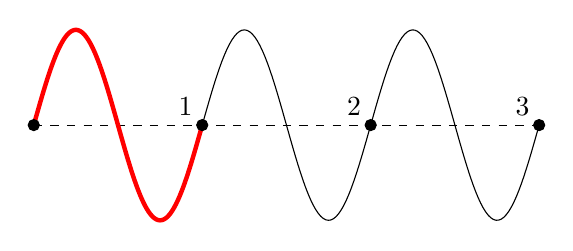
\begin{tikzpicture}
\begin{axis}[width=8cm,height=4cm,
    xmin=0,xmax=6,
    ymin=-1,ymax=1,
    clip=false,
    ticks=none,
    axis line style={draw=none}]
    \draw[dashed] (0,0) -- (6,0);
    \draw plot[domain=0:6*pi, samples=200] (\x/pi,{sin(\x r)});
    \draw[ultra thick, red] plot[domain=0:2*pi, samples=200] (\x/pi,{sin(\x r)});
    \draw[fill=black] (0,0) circle (2pt) 
        (2,0) circle (2pt) node[above left] {1}
        (4,0) circle (2pt) node[above left] {2}
        (6,0) circle (2pt) node[above left] {3};
\end{axis}
\end{tikzpicture}
\end{center}

\solutionEnd


\begin{example}
How many wave cycles are shown below? 
\end{example}

\begin{center}
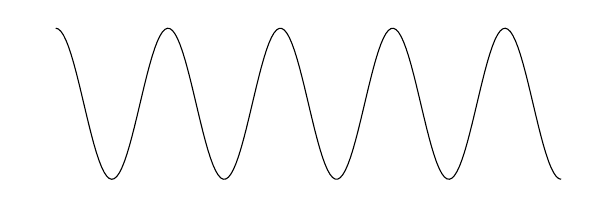
\begin{tikzpicture}
\begin{axis}[width=8cm,height=3.5cm,
    xmin=0,xmax=9,
    ymin=-1,ymax=1,
    clip=false,
    ticks=none,
    axis line style={draw=none}]
    \draw plot[domain=0.5*pi:0.5*pi + 4.5*2*pi, samples=200] (\x/pi,{sin(\x r)});
\end{axis}
\end{tikzpicture}
\end{center}


\Solution There are 4.5 wave cycles. Note that the 4th wave begins at a crest but finish a half-wave cycle later at a trough.



\begin{center}
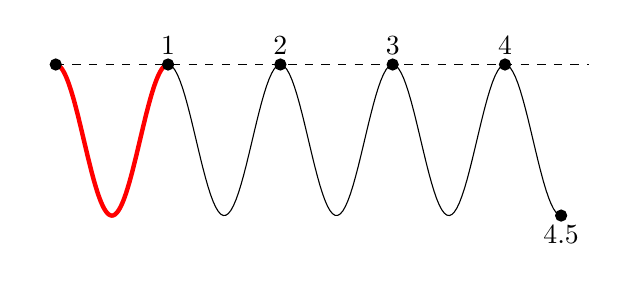
\begin{tikzpicture}
\begin{axis}[width=8cm,height=3.5cm,
    xmin=0,xmax=9,
    ymin=-1,ymax=1,
    clip=false,
    ticks=none,
    axis line style={draw=none}]
    \draw plot[domain=0.5*pi:0.5*pi + 4.5*2*pi, samples=200] (\x/pi,{sin(\x r)});
    \draw[ultra thick, red] plot[domain=0.5*pi:0.5*pi + 2*pi, samples=200] (\x/pi,{sin(\x r)});
    \draw[dashed] (0.5,1) -- ++ (axis direction cs: 0.5+4.5*2,0);
    \draw[fill=black] (0.5,1) circle (2pt)
        (0.5+2,1) circle (2pt) node[above] {1}
        (0.5+2*2,1) circle (2pt) node[above] {2}
        (0.5+3*2,1) circle (2pt) node[above] {3}
        (0.5+4*2,1) circle (2pt) node[above] {4}
        (0.5+4.5*2,-1) circle (2pt) node[below] {4.5};
\end{axis}
\end{tikzpicture}
\end{center}

\solutionEnd

\subsection*{\ref{ZAl8Xb} Exercises}

\begin{exercise}
How many wave cycles are shown below?

\begin{center}
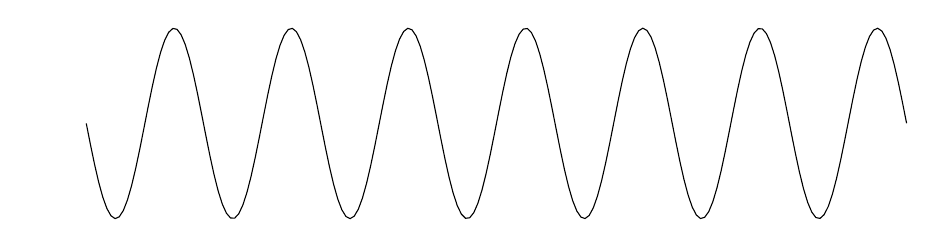
\begin{tikzpicture}
\begin{axis}[width=12cm,height=4cm,
    xmin=0,xmax=7*2,
    ymin=-1,ymax=1,
    clip=false,
    ticks=none,
    axis line style={draw=none}]
    \draw plot[domain=pi:pi+7*2*pi, samples=200] (\x/pi,{sin(\x r)});
\end{axis}
\end{tikzpicture}
\end{center}
\end{exercise}

\begin{exercise}
How many wave cycles are shown below?

\begin{center}
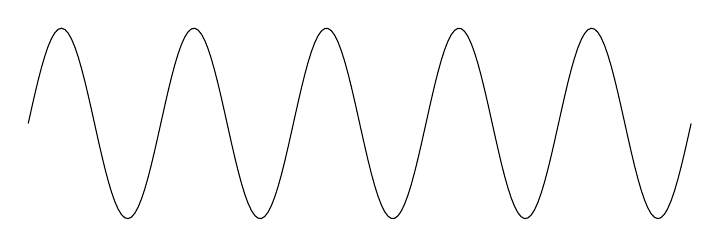
\begin{tikzpicture}
\begin{axis}[width=10cm,height=4cm,
    xmin=0,xmax=5*2,
    ymin=-1,ymax=1,
    clip=false,
    ticks=none,
    axis line style={draw=none}]
    \draw plot[domain=0:5*2*pi, samples=200] (\x/pi,{sin(\x r)});
\end{axis}
\end{tikzpicture}
\end{center}
\end{exercise}

\begin{exercise}
    How many wave cycles are shown below?

\begin{center}
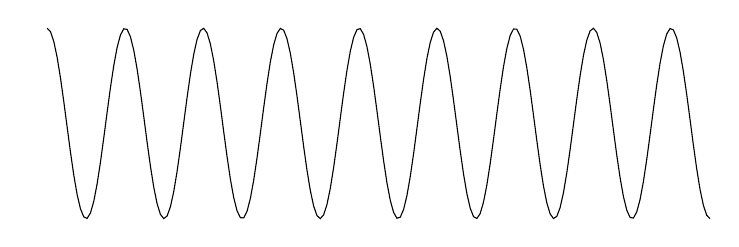
\begin{tikzpicture}
\begin{axis}[width=10cm,height=4cm,
    xmin=0,xmax=8.5*2,
    ymin=-1,ymax=1,
    clip=false,
    ticks=none,
    axis line style={draw=none}]
    \draw plot[domain=0.5*pi:0.5*pi + 8.5*2*pi, samples=200] (\x/pi,{sin(\x r)});
\end{axis}
\end{tikzpicture}
\end{center}
\end{exercise}

\begin{exercise}
    How many wave cycles are shown below?

\begin{center}
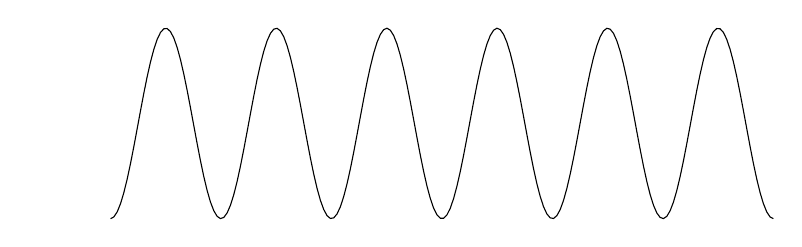
\begin{tikzpicture}
\begin{axis}[width=10cm,height=4cm,
    xmin=0,xmax=6*2,
    ymin=-1,ymax=1,
    clip=false,
    ticks=none,
    axis line style={draw=none}]
    \draw plot[domain=1.5*pi:1.5*pi + 6*2*pi, samples=200] (\x/pi,{sin(\x r)});
\end{axis}
\end{tikzpicture}
\end{center}
\end{exercise}

\begin{exercise}
    How many wave cycles are shown below?

\begin{center}
\begin{tikzpicture}
\begin{axis}[width=10cm,height=4cm,
    xmin=1,xmax=3.75*2,
    ymin=-1,ymax=1,
    clip=false,
    ticks=none,
    axis line style={draw=none}]
    \draw plot[domain=pi:pi + 3.75*2*pi, samples=200] (\x/pi,{sin(\x r)});
\end{axis}
\end{tikzpicture}
\end{center}
\end{exercise}

\cyanhrule

\subsection{Period and Frequency} \label{BcrbfW}
Because waves are in motion and travel from one place to another, we can study them with respect to time. A stopwatch is helpful for the following exercise. 

\begin{example} \label{GlVTg1}
    Access the \texttt[red]{PhET Simulation} ``Waves on a String'' (\href{https://phet.colorado.edu/en/simulations/wave-on-a-string}{click here}), to visualize the propagation of transverse waves. Then take the following steps.
    
    \begin{enumerate}
    \setlength\itemsep{0.1ex}
        \item Press the screen (on the play button) to start the simulation.
        \item Select the \texttt[red]{Oscillate} and \texttt[red]{No End} options.
        \item Increase \texttt[red]{Amplitude} to \SI{1.25}{cm}.
        \item Decrease \texttt[red]{Frequency} to \SI{0.50}{Hz}.
        \item Press the pause ({\tiny \faPause}) button at the instant the green bead on the end of the oscillating rod is at the highest point in the wave cycle (i.e. at the crest), as shown in Figure \ref{sAa4ih} below. Now press play ({\tiny \faPlay}) and observe this green bead travel from the crest, down to the trough, and back up to the crest. The amount of time it takes the bead to make this trip is known as the wave's \gls{period} of oscillation. 
        \item \label{82ffkH} Open the stopwatch app on your phone. Record 10 periods of the wave. In other words, measure the amount of time it takes the bead to make a 10 trips, each from crest, to trough, and back to crest. 
        \item \label{raDsYR} Divide the total time interval from the previous step by 10. The result is the average period of the wave as experimentally measurement by you.
        \item Repeat steps \ref{82ffkH} and \ref{raDsYR} for waves with frequencies of \SI{1.20}{Hz} and \SI{3.00}{Hz}. \textit{Note}: The higher the frequency, the more challenging it is for you to measure period.
    \end{enumerate}
    
    
\end{example}

\begin{center}
    \includegraphics[width=12cm]{figures/Unit11_PhET_Wave.png}
    \captionsetup{type=figure,margin=1in}
    \captionof{figure}{A screen shot from the ``Wave on a String'' \texttt{PhET Simulation}.}
    \label{sAa4ih}
\end{center}

\Solution For a wave with a frequency of \SI{0.50}{Hz}, the measured period is approximately 2 seconds. At frequencies of \SI{1.20}{Hz} and \SI{3.00}{Hz}, the periods are approximately \SI{0.8}{s} and \SI{0.3}{s}, respectively. You should notice that as the frequency of the wave increases, the period \textit{decreases}.

\solutionEnd

\vspace{1em}

Example \ref{GlVTg1} introduces two additional properties of waves: period and frequency. \Gls{period} is the time it takes to complete one wave cycle or oscillation. \Gls{frequency} is the number of wave cycles or oscillations completed in a time interval of 1 second. Period and frequency are \textit{inversely} related:

\begin{equation} \label{9WT68r}
    f = \frac{1}{T} \hspace{2em} 
    T = \frac{1}{f}
\end{equation}

By ``inversely'' related, we mean that as period increases, frequency decreases, and vice-verse. Period is measured in seconds. Frequency is measured in 1 over seconds, or Hertz (Hz). Thus, \SI{1}{Hz} is equivalent is 1/s.

\begin{center}
    \begin{tabular}{cl|cc}
    \hline
    \textbf{Symbol} & \textbf{Quantity} & \textbf{SI Base Unit} & \textbf{Unit Symbol}  \\
    \hline\hline
        $f$ & frequency & hertz & \si{\Hz}\\
        $T$ & period & second & s\\
    \hline
    \end{tabular}
\end{center}

\begin{example}
    A transverse wave completes 1 wave cycle every 0.25 seconds. What is the frequency of the wave?
\end{example}

\Solution We are given the period of the wave: $T = \SI{0.25}{s}$. By Equation \ref{9WT68r}, its frequency is

\begin{equation*}
    f = \frac{1}{T} = \frac{1}{0.25} = \SI{4}{\Hz}\ .
\end{equation*}

Therefore, this wave completes 4 wave cycles every second.

\solutionEnd

\begin{example}
    If a wave completes exactly $3 \frac{1}{3}$ wave cycles every second, what is the period of oscillation of the wave? 
\end{example}

\Solution We are given the wave's frequency as 3 and one-third hertz, or $f = 3\frac{1}{3}\,\text{Hz}$. This mixed number is written as an improper\footnote{See \href{https://openstax.org/books/prealgebra-2e/pages/4-1-visualize-fractions}{Section 4.1} of \textit{OpenStax: Prealgebra 2e} for a review on mixed numbers and improper fractions.} fraction as

\begin{equation*}
    3 \frac{1}{3} = \frac{10}{3} = 3.\overline{3}
\end{equation*}

So, the frequency is $f = \frac{10}{3}\,\text{Hz}$. The period, by Equation~\eqref{9WT68r}, is

\begin{equation*}
    T = \frac{1}{f} = \frac{1}{\frac{10}{3}} = \frac{3}{10}  = \SI{0.3}{s}
\end{equation*}

Therefore, it takes this wave 0.3 seconds to complete one wave cycle. 

\solutionEnd

\subsection*{\ref{BcrbfW} Exercises}

\begin{exercise} \label{XGViXs}
    The period of a wave is measured to be 4.85 seconds. What is the wave's frequency?
\end{exercise} 

\begin{exercise} \label{EeHAB4} 
    If the frequency of a wave is 8.53 hertz, what is its period of oscillation?
\end{exercise}

\begin{exercise} \label{ldTSm3} 
    A bead on a string oscillates between a crest and trough of a transverse wave. The bead completes 20 cycles in 16 seconds. Calculate the wave's average period of oscillation. 
\end{exercise}

\begin{exercise} \label{3rLSIq}
    What is the frequency of the wave described in Exercise \ref{ldTSm3}?
\end{exercise}

\begin{exercise} \label{gz0LQL} 
    Every second, a transverse wave completes exactly five and four-sevenths of a wave cycle. Calculate the period of oscillation.
\end{exercise}

\begin{exercise} \label{MITNpN} 
    Electromagnetic (EM) waves are transverse (but not mechanical) waves that oscillate at high frequencies. One type of EM waves is the radio wave, like those use detected by your car. Calculate the frequency of a radio wave whose period of oscillation is a tiny \SI[group-separator={\,}]{0.0001814}{s}.
\end{exercise}

\cyanhrule

\subsection{Wave Velocity} \label{nkz8rf}
Waves \gls{propagate}, or move in a given direction from their source. \Gls{wave velocity} ($v$) is the speed at which a wave propagates. To calculate wave velocity, you need only two quantities:

\begin{enumerate}
\setlength\itemsep{0.1ex}
    \item wavelength ($\lambda$)
    \item frequency ($f$)
\end{enumerate}

Wave velocity is frequency times wavelength:

\begin{equation} \label{UeynWL}
    v = f \lambda
\end{equation}


\begin{center}
    \begin{tabular}{cl|cc}
    \hline
    \textbf{Symbol} & \textbf{Quantity} & \textbf{SI Base Unit} & \textbf{Unit Symbol}  \\
    \hline\hline
        $v$ & wave velocity & meter per second & \si{\meter/\second}\\
        $f$ & frequency & hertz & \si{\Hz}\\
        $\lambda$ & wavelength & meter & m\\
    \hline
    \end{tabular}
    % \caption{Caption}
    \label{fig:Unit10_Table}
\end{center}

% \textit{PhET Simulation}: ``Waves Intro: Light'' (\href{https://phet.colorado.edu/sims/html/waves-intro/latest/waves-intro_en.html}{link})

\begin{example}
The frequency of a wave is 2.5 hertz, and its wavelength is 3.0 meters. Calculate the wave velocity.
\end{example}

\Solution We are given the frequency and wavelength: $f = \SI{2.5}{Hz}$ and $\lambda = \SI{3.0}{m}$. By Equation \eqref{UeynWL}, wave velocity is

\begin{equation*}
    v = f \lambda = (2.5)(3.0) = \SI{7.5}{m/s}
\end{equation*}

Thus, this wave moves at a speed of 7.5 meters per second.

\solutionEnd

\begin{example}
    The period of a wave is 0.78 seconds. Its wavelength is 1.1 meters. What is the wave's velocity?
\end{example}

\Solution We are given period and wavelength: $T = \SI{0.78}{s}$ and $\lambda = \SI{1.1}{m}$. The wave's frequency, by Equation \eqref{9WT68r}, is

\begin{equation*}
    f = \frac{1}{T} = \frac{1}{0.78} = \SI{1.28}{Hz}
\end{equation*}


Therefore, the wave velocity (Eq.~\ref{UeynWL}) is

\begin{equation*}
    v = f \lambda = (1.28)(1.1) = \SI{1.4}{m/s}
\end{equation*}

This wave travels at 1.4 meters per second.

\solutionEnd

\subsection*{\ref{nkz8rf} Exercises}

\begin{exercise}
    What two physical quantities are needed to calculate the velocity of a wave?
\end{exercise}

\begin{exercise} \label{SKv3ek}
    The following wave has a frequency of \SI{2.70}{Hz} and propagates to the right. What is the velocity of the wave?
\end{exercise}

\begin{center}
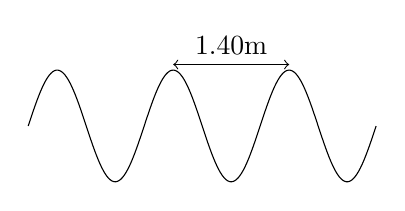
\begin{tikzpicture}
\begin{axis}[width=6cm,height=3cm,
    xmin=0,xmax=3*2,
    ymin=-1,ymax=1,
    clip=false,
    ticks=none,
    axis line style={draw=none}]
    \draw plot[domain=0:3*2*pi, samples=200] (\x/pi,{sin(\x r)});
    \draw[<->] (2.5,1.1) -- ++(axis direction cs: 2,0) node[above,pos=0.5] {\SI{1.40}{m}};
\end{axis}
\end{tikzpicture}
\end{center}


\begin{exercise} \label{HcdmDZ}
    The wave below has a period of 11 seconds as it propagates rightwards. Calculate its wave velocity.

\begin{center}
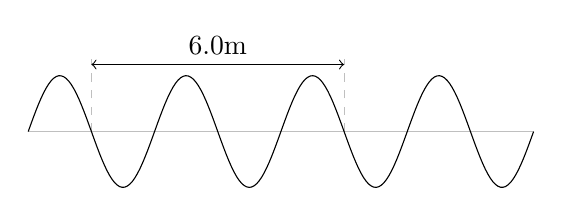
\begin{tikzpicture}
\begin{axis}[width=8cm,height=3cm,
    xmin=0,xmax=4*2,
    ymin=-1,ymax=1,
    clip=false,
    ticks=none,
    axis line style={draw=none}]
    \draw[lightgray] (0,0) -- (4*2,0);
    \draw[lightgray,dashed] (1,0) -- ++(axis direction cs: 0,1.3) (5,0) -- ++(axis direction cs: 0,1.3);
    \draw plot[domain=0:4*2*pi, samples=200] (\x/pi,{sin(\x r)});
    \draw[<->] (1,1.2) -- ++(axis direction cs: 4,0) node[above,pos=0.5] {\SI{6.0}{m}};
\end{axis}
\end{tikzpicture}
\end{center}
\end{exercise}

\begin{exercise} \label{exdA2j}
    Calculate the velocity of a wave whose wavelength and period of oscillation are \SI{10.5}{m} and \SI{0.25}{s}, respectively. 
\end{exercise}

\begin{exercise} \label{HoRqxe}
    What is the velocity of a wave whose frequency and wavelength are \SI{25}{Hz} and \SI{7.0}{m}, respectively?
\end{exercise}

\begin{exercise} \label{3zl6SU}
    Access the \texttt[red]{PhET Simulation} ``Waves Intro'' (\href{https://phet.colorado.edu/sims/html/waves-intro/latest/waves-intro_en.html}{click here}). Click the \texttt[red]{Light} panel. 

    \begin{enumerate}
    \setlength\itemsep{0.1ex}
        \item Press the \texttt[green!60!black]{green} button on the laser to emit green light waves.
        \item Click and drag the ruler tool from the upper-right-hand corner to measure the horizontal distance from the center of one bright spot to the next. \textbf{Tip}: by default, the ruler is set the measure the wavelength of green light.
        \item Convert the given measurement from nanometers (nm) to meters (m), given that $\SI{1}{nm} = 10^{-9}\,\text{m}$.
        \item If the wave travels at a speed of 300 million meters per second (\SI{3e8}{m/s}), what is the frequency of the light wave? Express the answer both in scientific notation and in decimal notation.
    \end{enumerate}


% \begin{center}
%     \includegraphics[width=12cm]{figures/Unit11_PhET_WavesIntro.png}
%     \captionsetup{type=figure,margin=1in,font=scriptsize}
%     \captionof{figure}{Screenshot of the \href{https://phet.colorado.edu/sims/html/waves-intro/latest/waves-intro_en.html}{Waves Intro} \texttt{PhET Simulation}. A ruler is used to measure the wavelength of a green laser.}
% \end{center}
\end{exercise}

\cyanhrule


\subsection{Superposition} \label{96T5dZ}

\begin{example} \label{OIqgoJ}
    Access the \texttt[red]{PhET Simulation} ``Waves on a String'' (\href{https://phet.colorado.edu/en/simulations/wave-on-a-string}{click here}). Then take the following steps two create two pulses.
    
    \begin{enumerate}
    \setlength\itemsep{0.1ex}
        \item Press the screen (on the play button) to start the simulation.
        \item Select the \texttt[red]{Pulse} and \texttt[red]{Loose End} options.
        \item Increase the \texttt[red]{Amplitude} to \SI{1.25}{cm}.
        \item Decrease the \texttt[red]{Damping} to \texttt[red]{None}.
        \item Set the \texttt[red]{Tension} to the medium value.
        \item Click the green pulse button twice, with a 1-second gap between the two clicks.
        \item When the two pulses overlap on the same side of the equilibrium line (above or below it), what happens to the string?
        \item When the two pulses are on opposite sides---for example, if one pulse is above the equilibrium line, and the other is below---what happens to the string?
    \end{enumerate}

    \begin{center}
        \includegraphics[width=12cm]{figures/Unit11_PhET_Wave2.png}
    \end{center}
\end{example}

\Solution When two pulses converge on the same side of the equilibrium line, that portion of the string grows in height as the amplitudes of the two pulses add up. However, when pulses that are on opposite sides converge, the string momentarily flattens as the opposite amplitudes of the pulses cancel each other out.

\solutionEnd

\vspace{1em}

The effect that we saw in Example \ref{OIqgoJ} is called superposition. \Gls{superposition} is the summation phenomenon that occurs when two waves arrive at the same point. 

\begin{center}
    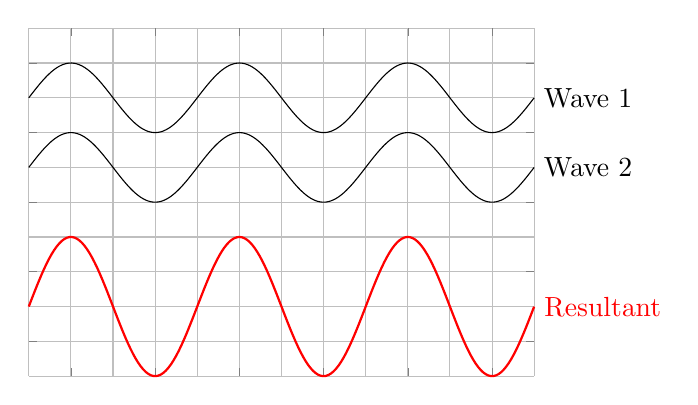
\begin{tikzpicture}[declare function={f(\x)=sin(\x r);},
        declare function={g(\x)=cos(\x r);}]
    \begin{axis}[width=8cm,height=6cm,
        xmin=0,xmax=6,
        ymin=-8,ymax=2,
        clip=false,
        minor tick num=1,
        ticks=none,
        axis line style={draw=none},
        grid=both,
    ]
    \draw[domain=0:6*pi,variable=\x,samples=200] plot ({\x/pi},{f(\x)}) node[right]{Wave 1};
    \draw[domain=0:6*pi,variable=\x,samples=200] plot ({\x/pi},{f(\x) - 2}) node[right] {Wave 2};
    \draw[red,thick,domain=0:6*pi,variable=\x,samples=200] plot ({\x/pi},{f(\x) + f(\x) - 6.0}) node[right] {Resultant};
    \end{axis}
    \end{tikzpicture}
\end{center}

\begin{center}
    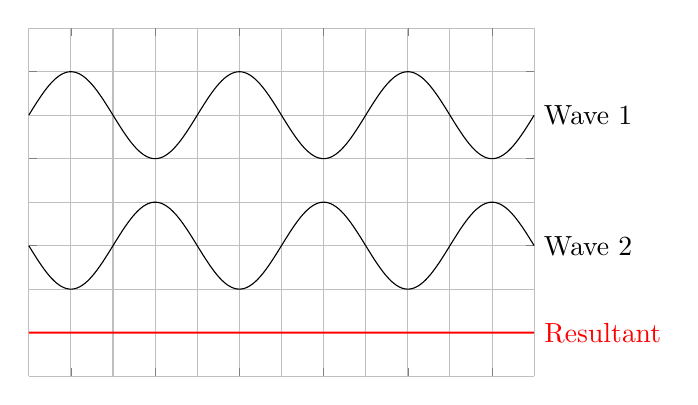
\begin{tikzpicture}[declare function={f(\x)=sin(\x r);},
        declare function={g(\x)=cos(\x r);}]
    \begin{axis}[width=8cm,height=6cm,
        xmin=0,xmax=6,
        ymin=-6,ymax=2,
        clip=false,
        minor tick num=1,
        ticks=none,
        axis line style={draw=none},
        grid=both,
    ]
    \draw[domain=0:6*pi,variable=\x,samples=200] plot ({\x/pi},{f(\x)}) node[right]{Wave 1};
    \draw[domain=0:6*pi,variable=\x,samples=200] plot ({\x/pi},{f(\x - pi) - 3}) node[right] {Wave 2};
    \draw[red,thick,domain=0:6*pi,variable=\x,samples=200] plot ({\x/pi},{f(\x) + f(\x-pi) - 5}) node[right] {Resultant};
    \end{axis}
    \end{tikzpicture}
\end{center}

\begin{center}
    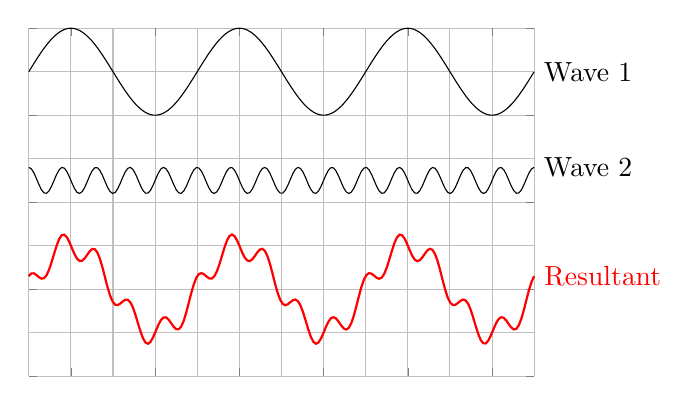
\begin{tikzpicture}[declare function={f(\x)=sin(\x r);},
        declare function={g(\x)=0.3*cos(\x*5 r);}]
    \begin{axis}[width=8cm,height=6cm,
        xmin=0,xmax=6,
        ymin=-7,ymax=1,
        clip=false,
        minor tick num = 1,
        ticks=none,
        axis line style={draw=none},
        grid=both,
    ]
    \draw[domain=0:6*pi,variable=\x,samples=200] plot ({\x/pi},{f(\x)}) node[right]{Wave 1};
    \draw[domain=0:6*pi,variable=\x,samples=200] plot ({\x/pi},{g(\x) - 2.5}) node[right] {Wave 2};
    \draw[red,thick,domain=0:6*pi,variable=\x,samples=200] plot ({\x/pi},{f(\x) + g(\x) - 5.0}) node[right] {Resultant};
    \end{axis}
    \end{tikzpicture}
    \captionsetup{type=figure,margin=1in}
    \captionof{figure}{Various examples of superposition.}
\end{center}

\subsection*{\ref{96T5dZ} Exercises}

{\color{white}{

\begin{exercise} \label{gbJp6v} 
\end{exercise} 

\vspace{-1cm}

\begin{exercise} \label{8e1BSx} 
\end{exercise} 

\vspace{-1cm}

\begin{exercise} \label{oRb52g} 
\end{exercise} 

\vspace{-1cm}

\begin{exercise} \label{vTVEZJ} 
\end{exercise} 

\vspace{-1cm}

\begin{exercise} \label{nd0J3q} 
\end{exercise} 

\vspace{-1cm}

\begin{exercise} \label{OCQiEo} 
\end{exercise}
}}

\textbf{\ref{gbJp6v}--\ref{OCQiEo}}. Consider two pulses on a string, one moving to the right, the other to the left. Each pulse moves at a rate of one unit grid per second. Draw the string at 1-second time intervals after the initial snapshot, using the principle of superposition to either add or subtract the amplitudes of the pulses when they overlap. \textit{Tip}: Use two colored pencils of different colors to shade the area under each pulse.


\clearpage

\begin{center}
    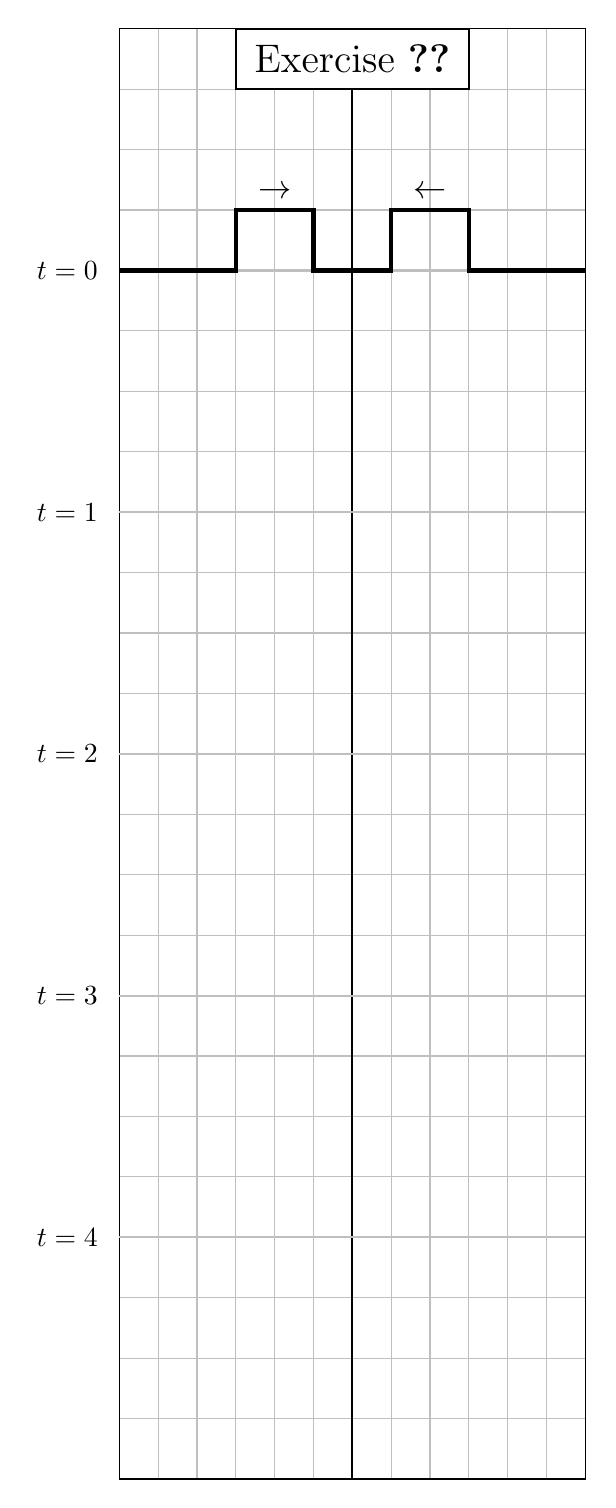
\begin{tikzpicture}
        \begin{axis}[width=7.5cm,height=20cm,
            xmin=0,xmax=12,
            ymin=0,ymax=24,
            ytick={0,1,...,24},
            xtick={0,1,...,12},
            grid=both,
            % minor tick num=1,
            ticks=none,
            clip=false,
        ]
            \draw[thick] (6,0) -- ++(0,24);
            \pgfplotsinvokeforeach{4,8,...,20}{
                \draw[lightgray,thick] (0,#1) -- ++ (12,0);
                }
            \node[left=1ex] at (0,4) {$t=4$};
            \node[left=1ex] at (0,8) {$t=3$};
            \node[left=1ex] at (0,12) {$t=2$};
            \node[left=1ex] at (0,16) {$t=1$};
            \node[left=1ex] at (0,20) {$t=0$};
            \draw[ultra thick] (0,20) -- ++(3,0) -- ++(0,1) -- ++(2,0) node[above,pos=0.5] {\large $\rightarrow$} -- ++(0,-1) -- ++(2,0) -- ++(0,1) -- ++(2,0) node[above,pos=0.5] {\large $\leftarrow$} -- ++(0,-1) -- ++(3,0);
        \draw[thick,fill=white] (3,23) rectangle ++(6,1) node[black,pos=0.5] {\Large Exercise \ref{gbJp6v}};
        \end{axis}
    \end{tikzpicture}%
    \hspace{2mm}
    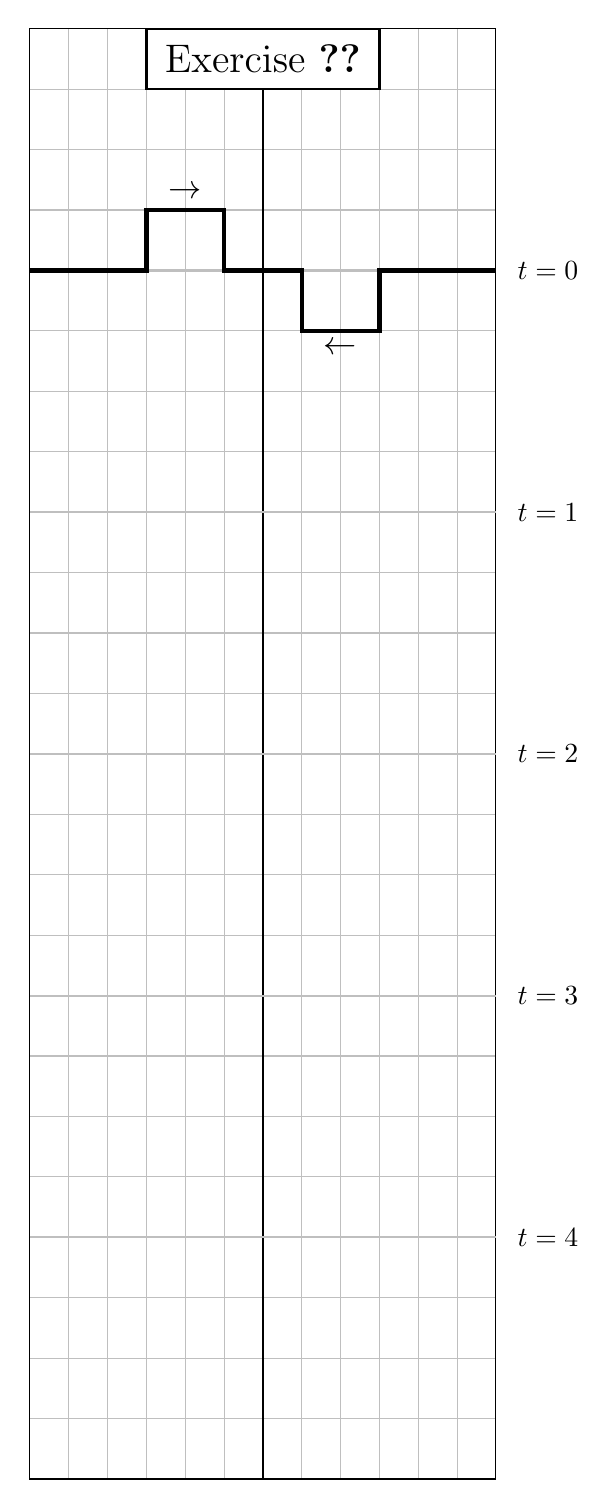
\begin{tikzpicture}
        \begin{axis}[width=7.5cm,height=20cm,
            xmin=0,xmax=12,
            ymin=0,ymax=24,
            ytick={0,1,...,24},
            xtick={0,1,...,12},
            grid=both,
            % minor tick num=1,
            ticks=none,
            clip=false,
        ]
            \draw[thick] (6,0) -- ++(0,24);
            \pgfplotsinvokeforeach{4,8,...,20}{
                \draw[lightgray,thick] (0,#1)  -- ++ (12,0);
                }
            \node[right=1ex] at (12,4) {$t=4$};
            \node[right=1ex] at (12,8) {$t=3$};
            \node[right=1ex] at (12,12) {$t=2$};
            \node[right=1ex] at (12,16) {$t=1$};
            \node[right=1ex] at (12,20) {$t=0$};
            \draw[ultra thick] (0,20) -- ++(3,0) -- ++(0,1) -- ++(2,0) node[above,pos=0.5] {\large $\rightarrow$} -- ++(0,-1) -- ++(2,0) -- ++(0,-1) -- ++(2,0) node[below,pos=0.5] {\large $\leftarrow$} -- ++(0,1) -- ++(3,0);
        \draw[thick,fill=white] (3,23) rectangle ++(6,1) node[black,pos=0.5] {\Large Exercise \ref{8e1BSx}};
        \end{axis}
    \end{tikzpicture}
\end{center}

\clearpage

\begin{center}
    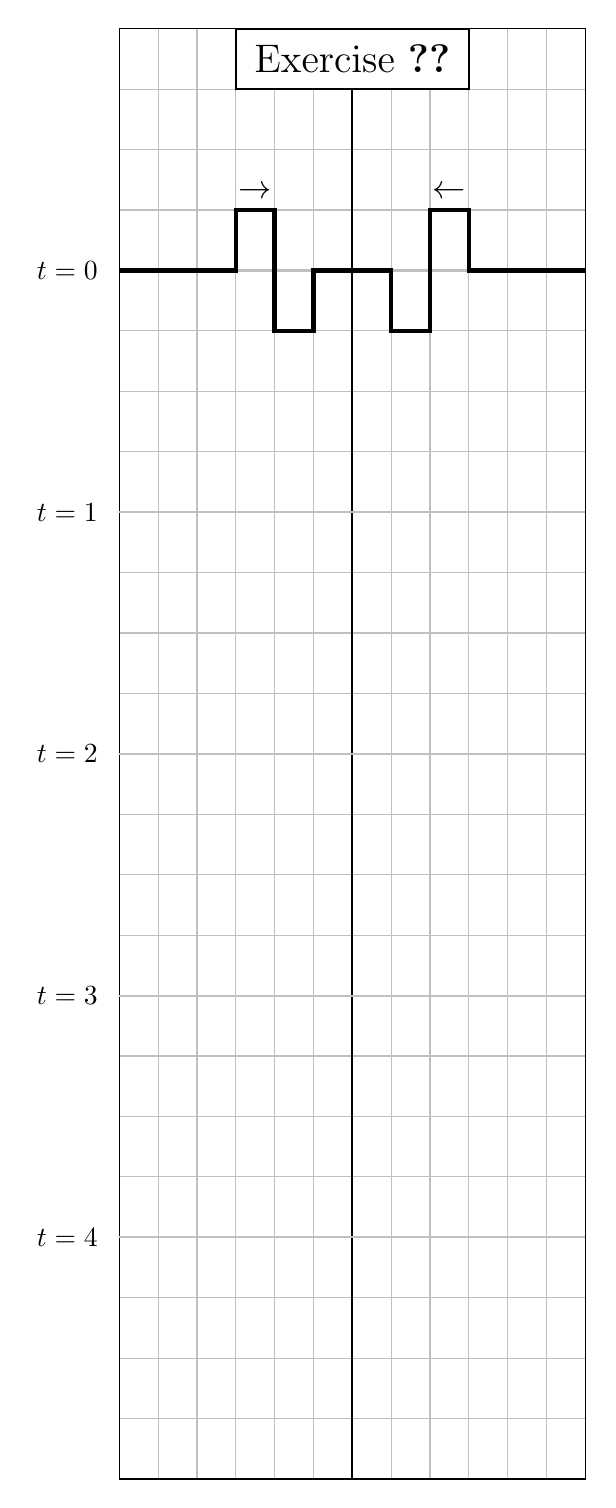
\begin{tikzpicture}
        \begin{axis}[width=7.5cm,height=20cm,
            xmin=0,xmax=12,
            ymin=0,ymax=24,
            ytick={0,1,...,24},
            xtick={0,1,...,12},
            grid=both,
            % minor tick num=1,
            ticks=none,
            clip=false,
        ]
            \draw[thick] (6,0) -- ++(0,24);
            \pgfplotsinvokeforeach{4,8,...,20}{
                \draw[lightgray,thick] (0,#1) -- ++ (12,0);
                }
            \node[left=1ex] at (0,4) {$t=4$};
            \node[left=1ex] at (0,8) {$t=3$};
            \node[left=1ex] at (0,12) {$t=2$};
            \node[left=1ex] at (0,16) {$t=1$};
            \node[left=1ex] at (0,20) {$t=0$};
            \draw[black,ultra thick] (0,20) -- ++(3,0) -- ++(0,1) -- ++(1,0) node[above,pos=0.5] {\large $\rightarrow$} -- ++(0,-2) -- ++(1,0) -- ++(0,1) -- ++(2,0) -- ++(0,-1) -- ++ (1,0) -- ++(0,2) -- ++(1,0) node[above,pos=0.5] {\large $\leftarrow$} -- ++(0,-1) -- ++(3,0);
        \draw[thick,fill=white] (3,23) rectangle ++(6,1) node[black,pos=0.5] {\Large Exercise \ref{oRb52g}};
        \end{axis}
    \end{tikzpicture}%
    \hspace{2mm}
    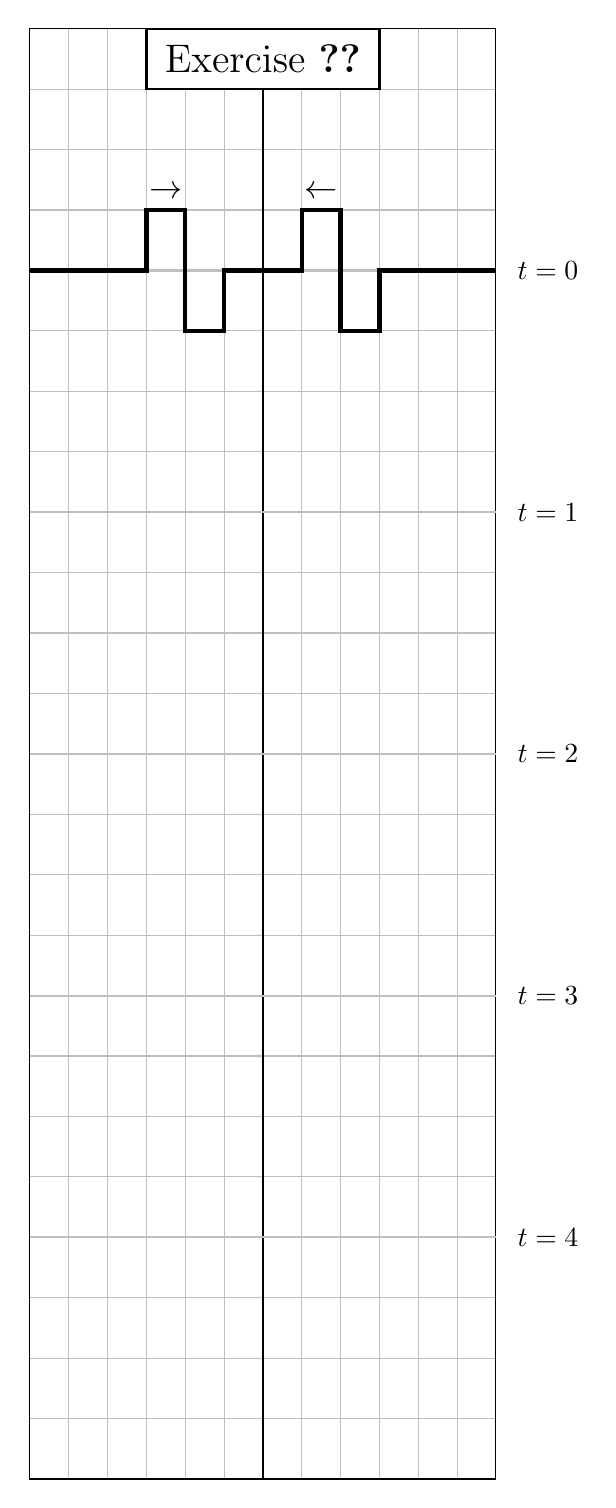
\begin{tikzpicture}
        \begin{axis}[width=7.5cm,height=20cm,
            xmin=0,xmax=12,
            ymin=0,ymax=24,
            ytick={0,1,...,24},
            xtick={0,1,...,12},
            grid=both,
            % minor tick num=1,
            ticks=none,
            clip=false,
        ]
            \draw[thick] (6,0) -- ++(0,24);
            \pgfplotsinvokeforeach{4,8,...,20}{
                \draw[lightgray,thick] (0,#1)  -- ++ (12,0);
                }
            \node[right=1ex] at (12,4) {$t=4$};
            \node[right=1ex] at (12,8) {$t=3$};
            \node[right=1ex] at (12,12) {$t=2$};
            \node[right=1ex] at (12,16) {$t=1$};
            \node[right=1ex] at (12,20) {$t=0$};
        \draw[black,ultra thick] (0,20) -- ++(3,0) -- ++(0,1) -- ++(1,0) node[above,pos=0.5] {\large $\rightarrow$} -- ++(0,-2) -- ++(1,0) -- ++(0,1) -- ++(2,0) -- ++(0,1) -- ++(1,0) node[above,pos=0.5] {\large $\leftarrow$} -- ++(0,-2) -- ++(1,0) -- ++(0,1) -- ++(3,0);
        \draw[thick,fill=white] (3,23) rectangle ++(6,1) node[black,pos=0.5] {\Large Exercise \ref{vTVEZJ}};
        \end{axis}
    \end{tikzpicture}
\end{center}

\clearpage

\begin{center}
    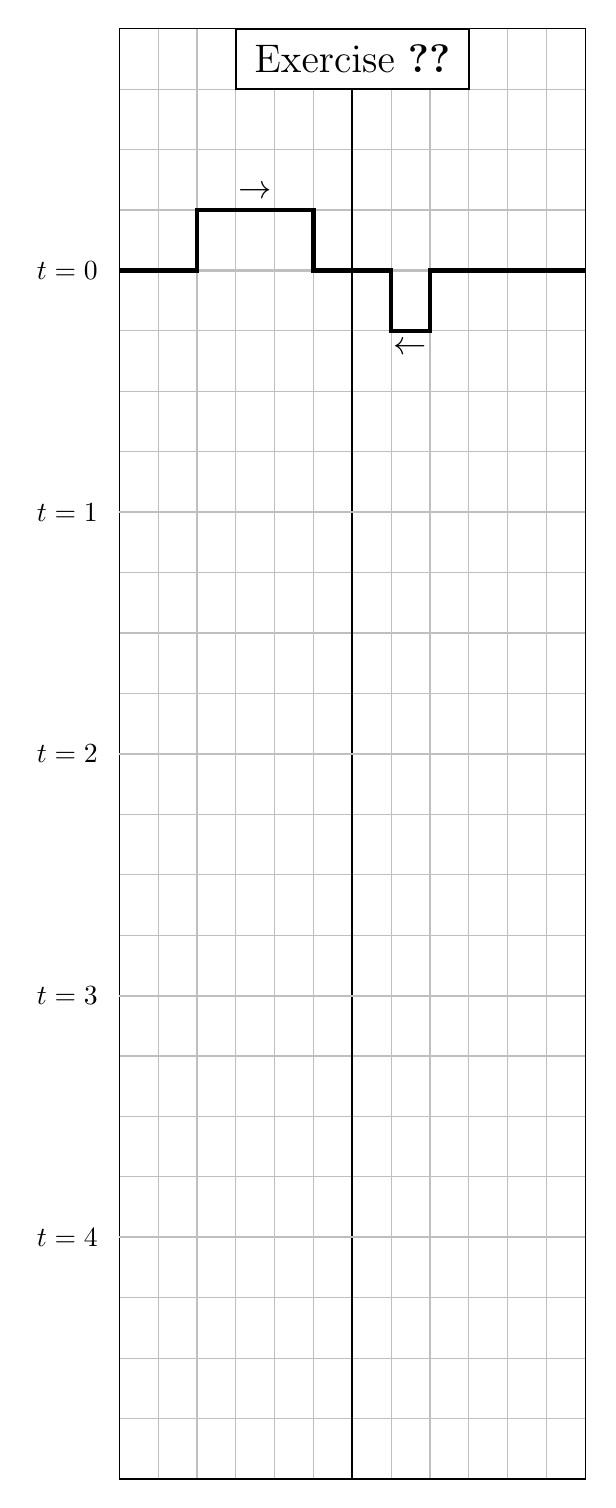
\begin{tikzpicture}
        \begin{axis}[width=7.5cm,height=20cm,
            xmin=0,xmax=12,
            ymin=0,ymax=24,
            ytick={0,1,...,24},
            xtick={0,1,...,12},
            grid=both,
            % minor tick num=1,
            ticks=none,
            clip=false,
        ]
            \draw[thick] (6,0) -- ++(0,24);
            \pgfplotsinvokeforeach{4,8,...,20}{
                \draw[lightgray,thick] (0,#1) -- ++ (12,0);
                }
            \node[left=1ex] at (0,4) {$t=4$};
            \node[left=1ex] at (0,8) {$t=3$};
            \node[left=1ex] at (0,12) {$t=2$};
            \node[left=1ex] at (0,16) {$t=1$};
            \node[left=1ex] at (0,20) {$t=0$};
            \draw[ultra thick] (0,20) -- ++(2,0) -- ++(0,1) -- ++(3,0) node[above,pos=0.5] {\large $\rightarrow$} -- ++(0,-1) -- ++(2,0) -- ++(0,-1) -- ++(1,0) node[below,pos=0.5] {\large $\leftarrow$} -- ++(0,1) -- ++(4,0);
        \draw[thick,fill=white] (3,23) rectangle ++(6,1) node[black,pos=0.5] {\Large Exercise \ref{nd0J3q}};
        \end{axis}
    \end{tikzpicture}%
    \hspace{2mm}
    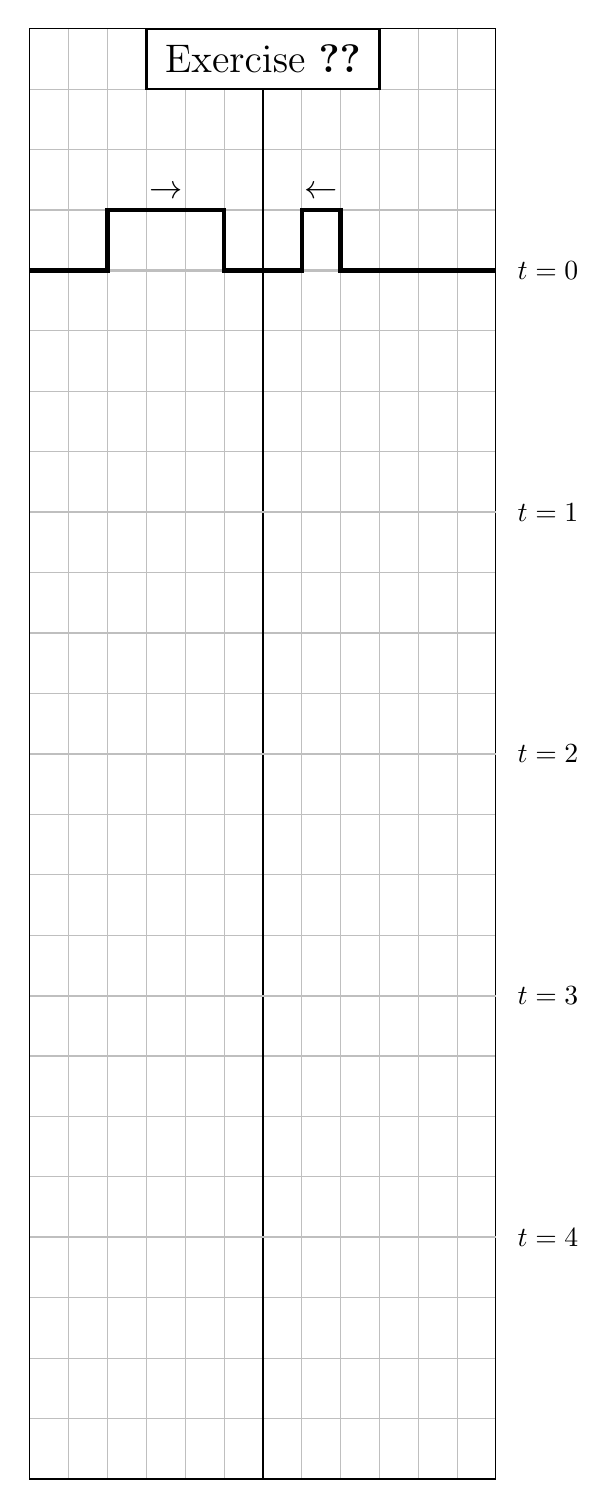
\begin{tikzpicture}
        \begin{axis}[width=7.5cm,height=20cm,
            xmin=0,xmax=12,
            ymin=0,ymax=24,
            ytick={0,1,...,24},
            xtick={0,1,...,12},
            grid=both,
            % minor tick num=1,
            ticks=none,
            clip=false,
        ]
            \node[right=1ex] at (12,4) {$t=4$};
            \node[right=1ex] at (12,8) {$t=3$};
            \node[right=1ex] at (12,12) {$t=2$};
            \node[right=1ex] at (12,16) {$t=1$};
            \node[right=1ex] at (12,20) {$t=0$};
            \draw[thick] (6,0) -- ++(0,24);
            \pgfplotsinvokeforeach{4,8,...,20}{
                \draw[lightgray,thick] (0,#1)  -- ++ (12,0);
                }
            \draw[black,ultra thick] (0,20) -- ++(2,0) -- ++(0,1) -- ++(3,0) node[above,pos=0.5] {\large $\rightarrow$} -- ++(0,-1) -- ++(2,0) -- ++(0,1) -- ++(1,0) node[above,pos=0.5] {\large $\leftarrow$} -- ++(0,-1) -- ++(4,0);
        \draw[thick,fill=white] (3,23) rectangle ++(6,1) node[black,pos=0.5] {\Large Exercise \ref{OCQiEo}};
        \end{axis}
    \end{tikzpicture}
\end{center}

\clearpage
\subsection{Longitudinal Waves and Sound} \label{FpyvAr}

\begin{center}
    \tikzset{declare function={f(\x)=sin(540*\x);}}
    \begin{tikzpicture}
     \draw[thick,-latex] (-0.5,0) -- (10,0)node[anchor=north west] {\gls{wave velocity}};
     \draw[very thick, domain=0.1:9.5,variable=\x,samples=500] plot
     ({\x-1.1*exp(-(\x-2)*(\x-2))-1.1*exp(-(\x-8)*(\x-8))},{f(\x)});
     \draw[latex-latex, thick] (0.6,1.5) -- (6.5,1.5) node[midway,above]{\gls{wavelength}};
     \draw[<->, thick]      (-1.7,0.3) node[left] {disturbance} --  + (1,0);
     \draw[->, thick]      (-1.7,-0.5) node[left] {propagation} -- + (1,0);
    \end{tikzpicture}
    \captionsetup{type=figure,margin=1in}
    \captionof{figure}{A longitudinal wave.}
    \label{fig:my_label}
\end{center}

A \gls{longitudinal wave} is a wave in which the disturbance is \textit{parallel} to the direction of propagation. Although they are invisible, sound waves are a great example of longitudinal waves. \Gls{sound} is a disturbance of matter that is transmitted from its source outward by longitudinal waves. The solid, liquid, or gas material through which a sound waves propagates is called the \gls{medium}. For example, if sound propagates from a speaker through the air in a room, then air is the medium. If you could see the air particles in the room during the propagation of a sound wave, you would see something like what is shown in Figure \ref{kfXDSQ}.

\begin{center}
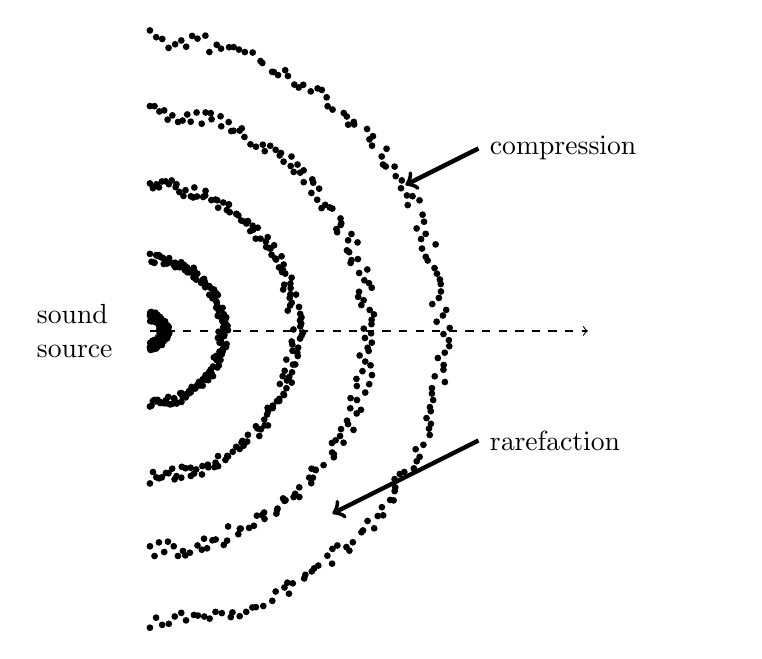
\begin{tikzpicture}
\begin{axis}[height=9cm,width=9cm,
  cycle list={
    only marks,mark size=1pt\\
    only marks,mark size=1pt\\
  },
  xmin=0,xmax=8,
  ymin=-4,ymax=4,
  domain=270:360+90,
  samples=150,
  axis line style={draw=none},
  ticks=none,
  clip=false,
]
\draw[dashed,->] (0,0) -- (6,0);
\addplot ({(0.2+0.07*rand)*cos(x)},{(0.2+0.07*rand)*sin(x)});
\addplot ({(1.0+0.07*rand)*cos(x)},{(1.0+0.07*rand)*sin(x)});
\addplot ({(2.0+0.10*rand)*cos(x)},{(2.0+0.10*rand)*sin(x)});
\addplot ({(3.0+0.12*rand)*cos(x)},{(3.0+0.12*rand)*sin(x)});
\addplot ({(4.0+0.12*rand)*cos(x)},{(4.0+0.12*rand)*sin(x)});

\draw[<-,ultra thick] (3.5,2) -- ++(axis direction cs: 1,0.5) node[right] {compression};
\draw[<-,ultra thick] (2.5,-2.5) -- ++(axis direction cs: 2,1) node[right] {rarefaction};

\node[align=left,left=1em] at (0,0) {sound\\ source};

\end{axis}
\end{tikzpicture}
\captionsetup{type=figure,margin=1in}
\captionof{figure}{Visualization of a sound wave propagating through air particles.}
\label{kfXDSQ}
\end{center}

%periodic variations

Sound waves cause a disturbance in the density and pressure of the surrounding air through which they propagate. What is density? \Gls{density} is the amount of matter or particles contained in a given region of space. If there are more air particles in a box, the region has a higher density compared to the same box with less particles, as shown below:

\begin{center}
    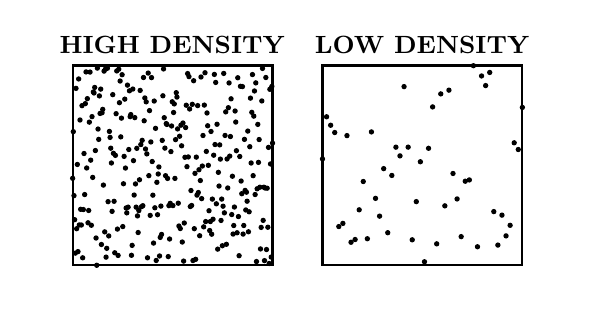
\begin{tikzpicture}[
        declare function={a(\x)=0*\x+2;},
        declare function={b(\x)=0*\x;}
    ]
    \begin{axis}[
        domain=0:5,
        axis lines=middle,
        axis equal image,
        xtick=\empty, ytick=\empty,
        axis line style={draw=none},
        enlargelimits=true,
        clip mode=individual, clip=false
    ]
    \addplot [black, only marks, mark=*, samples=300, mark size=0.75,domain=0:2]
        {0.5*(a(x)+b(x)) + 0.5*rand*(a(x)-b(x))};
        
    \addplot [black, only marks, mark=*, samples=50, mark size=0.75,domain=2.5:4.5]
        {0.5*(a(x)+b(x)) + 0.5*rand*(a(x)-b(x))};
    \draw[thick] (axis cs: 0,0) rectangle (axis cs: 2,2);
    \draw[thick] (axis cs: 2.5,0) rectangle (axis cs: 4.5,2);
    \node at (axis cs: 1,2.2) {\small \textbf{HIGH DENSITY}};
    \node at (axis cs: 3.5,2.2) {\small \textbf{LOW DENSITY}};
    \end{axis}
    \end{tikzpicture}
    \captionsetup{type=figure,margin=1in,font=scriptsize}
    \captionof{figure}{Particles in two boxes of identical size. The air density is higher in the box with more particles.}
\end{center}


\Gls{pressure} is the force applied by air molecules over a given surface area. High-density regions of air exert more pressure than comparatively lower density regions. As seen in Figure \ref{kfXDSQ}, sound waves consists of periodic variations in air density---and, therefore, air pressure---and these variations propagate as longitudinal waves. A high-pressure (high-density) region of a sound wave is called a \gls{compression}, and a low-pressure region is called a \gls{rarefaction}. \Gls{atmospheric pressure} is the normal pressure of the air due to Earth's atmosphere, and compressions of a sound wave are slightly above atmospheric pressure. Rarefactions are below atemospheric pressure. 

\vspace{1em}

See the horizontal dashed line in Figure \ref{kfXDSQ}? If you plot the air pressure as a function of distance from the sound source across the dashed line, you get the plot shown in Figure \ref{6cfkhd} below. This ``gauge pressure'' is an excellent visualization of how a sound wave varies both above and below atmospheric pressure.
\vspace{1em}

% Standard atmospheric pressure is defined as $P_{\text{atm}} = \SI{1}{atm} = \SI{101.3}{kPa}$. Sound waves produce periodic variations slightly above and below atmospheric pressure. Periodic variations in pressure are shown below.

\begin{center}
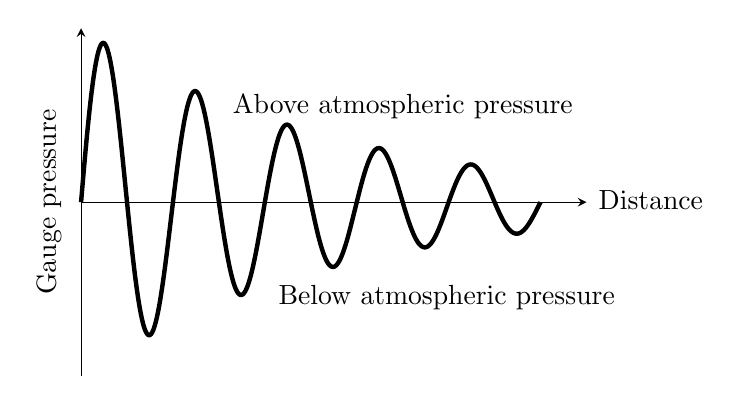
\begin{tikzpicture}
\begin{axis}[width=8cm,height=6cm,
    axis lines = center,
    xlabel = {Distance},
    ylabel = {Gauge pressure},
    xtick=\empty, ytick=\empty,
    ymin=-1, ymax=1,
    x label style={at={(axis description cs:1.25,0.45)}},
    y label style={at={(axis description cs:-0.02,.5)},rotate=90,anchor=south},
    xmax = 11*pi,
    clip=false,
]
\addplot [ultra thick,
    domain=0:2*pi*5, 
    samples=500, 
    color=black,
]
{sin(deg(x))*exp(deg(-x*0.001))};
\node at (22,0.55) {Above atmospheric pressure};
\node at (25,-0.55) {Below atmospheric pressure};
\end{axis}
\end{tikzpicture}
\captionsetup{margin=1in,type=figure,font=small}
\captionof{figure}{The graph shows gauge pressure versus distance from a sound source. Gauge pressure is the pressure relative to atmospheric pressure; it is positive for pressures above atmospheric pressure, and negative for pressures below it. For ordinary, everyday sounds, pressures vary only slightly from average atmospheric pressure.}
\label{6cfkhd} 
\end{center}

Noise-cancelling headphones (like AirPods) work by duplicating a sound wave of the external environment and shifting the duplicate out of phase with the original wave. In order words, the compressions of the original wave are perfectly aligned with the rarefactions of the duplicate. The duplicate may be called ``anti-noise,'' since, by superposition, it effectively cancels out the external sound. See Figure \ref{r1JrlI}.


\begin{center}
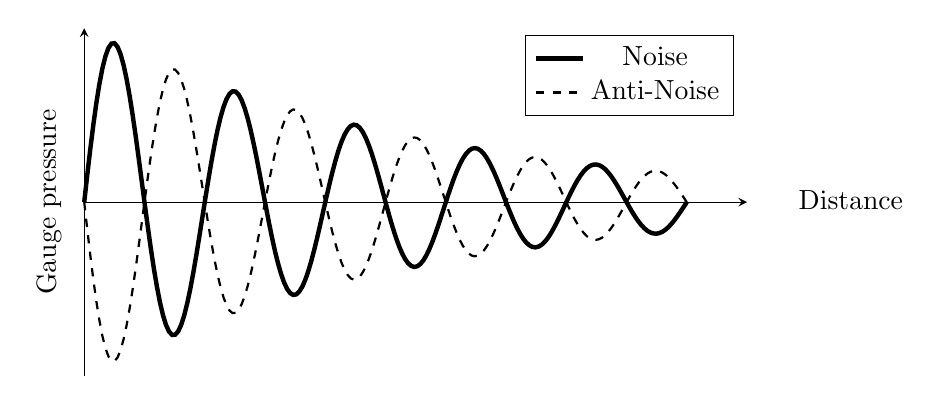
\begin{tikzpicture}
\begin{axis}[width=10cm,height=6cm,
    axis lines = center,
    xlabel = {Distance},
    ylabel = {Gauge pressure},
    xtick=\empty, ytick=\empty,
    ymin=-1, ymax=1,
    x label style={at={(axis description cs:1.25,0.45)}},
    y label style={at={(axis description cs:-0.02,.5)},rotate=90,anchor=south},
    xmax = 11*pi,
    clip=false,
]
\addplot [ultra thick,
    domain=0:2*pi*5, 
    samples=200, 
    color=black,
]
{sin(deg(x))*exp(deg(-x*0.001))};
\addlegendentry{Noise};

\addplot [thick,dashed,
    domain=0:2*pi*5, 
    samples=200,
]
{-sin(deg(x))*exp(deg(-x*0.001))};
\addlegendentry{Anti-Noise};
\end{axis}
\end{tikzpicture}
\captionsetup{margin=1in,type=figure,font=scriptsize}
\captionof{figure}{How noise-cancelling headphones work.}
\label{r1JrlI}
\end{center}


We conclude with a note on the speed of sound. Sound speed depends on the medium. The speed of a sound wave propagating through air---the medium most commonly associated with sound---is 331 meters per second (about \SI{740}{mph}). Sound travels at different speeds through different media, like water, carbon dioxide, or glass. However, it does not propagate through a vacuum (i.e. empty space), since sound requires a medium through which the longitudinal wave may travel.

\subsection*{\ref{FpyvAr} Exercises}

\begin{exercise}
    Define the following words: longitudinal wave, sound, medium, compression, rarefaction, atmospheric pressure. 
\end{exercise}

\begin{exercise} \label{AZF19g}
     Bring Figure \ref{kfXDSQ} alive by operating the \texttt[red]{PhET Simulation} ``Waves Intro'' (\href{https://phet.colorado.edu/sims/html/waves-intro/latest/waves-intro_en.html}{click here}). Select the middle panel, labeled \texttt[red]{Sound}.
    
     \begin{enumerate}
     \setlength\itemsep{0.1ex}
        \item Select the \texttt[red]{Both} option.
        \item Press the \texttt[green!70!black]{green} button to emit sound waves.
        \item Compare the simulation with Figure \ref{kfXDSQ}. Draw a quick sketch of your screen.
     \end{enumerate}
\end{exercise}

\begin{exercise}
    Bring Figure \ref{6cfkhd} to life. Follow all the steps in Exercise \ref{AZF19g}. Then check the \texttt[red]{Graph} box. Draw a quick sketch of what you see. 
\end{exercise}

\begin{exercise}
    Between a compression and a rarefaction, which is below atmospheric pressure?
\end{exercise}

\begin{exercise}
    Name the part of a sound wave that is slightly above atmospheric pressure.
\end{exercise}

\begin{exercise}
    Watch ``How Do Noise Canceling Headphones Work?'' by \texttt{Branch Education} on \texttt{YouTube} (\href{https://youtu.be/VIi04uD8LtY}{click here}). In your own words, briefly summarize how noise-cancelling headphones work. Use the terms defined in this section.
\end{exercise}

\begin{exercise} \label{J5ZJhe}
    Whales emit deep sounds through the ocean. Find Table 14.1 in \texttt[red]{OpenStax: Physics} (\href{https://openstax.org/books/physics/pages/14-1-speed-of-sound-frequency-and-wavelength#Table_14_01}{click here}). What is the speed of a sound wave through sea water? Between air and water, through which medium does sound travel faster?
\end{exercise}

\begin{exercise}
    Access the table from Exercise \ref{J5ZJhe}. Identify the media through which sound waves travel the slowest and the fastest.
\end{exercise}







\clearpage

\subsection*{Additional Resources}

\begin{itemize}
    \item \texttt{YouTube}: ``Transverse wave using slinky coil'' by \texttt{Evan Toh} (\href{https://youtu.be/g8GcMn7K0u4}{click here}). Sound waves are NOT transverse waves.
    \item \texttt{YouTube}: ``Longitudinal wave using slinky coil'' (\href{https://youtu.be/fMJrtheQfZw}{click here}). Sound waves are longitudinal waves that travel through matter.
    \item \textit{Cosmos}: Season 1, Episode 5: ``Hiding in the Light'' (\href{https://www.amazon.com/Cosmos-Spacetime-Odyssey-Season-1/dp/B00IHCHOGQ}{click here}). See min.~(25:40)--(28:18) for visualization of sound waves.
    \item \texttt{PhET Simulation}:  ``Waves Intro: Sound'' (\href{https://phet.colorado.edu/sims/html/waves-intro/latest/waves-intro_en.html}{click here}). Click the \texttt[red]{Sound} panel. Check \texttt[red]{Play Tone} and \texttt[red]{Both}, and then press the green button on the speaker. This is a visual of sound waves.
    \item \texttt{PhET Simulation}: ``Gas Properties'' (\href{https://phet.colorado.edu/sims/html/gas-properties/latest/gas-properties_en.html}{click here}). Select \texttt[red]{Ideal} panel. For an example of density, hold volume constant and add particles to the container.
    \texttt{PhET Simulation}: ``Sound'' (\href{https://phet.colorado.edu/en/simulations/sound}{click here})
    \item \texttt{YouTube}: ``AirPods Max---Hear What It Actually Sounds Like'' by \texttt{iPhonedo} (\href{https://youtu.be/97gTzS9VFxo?t=134}{click here}). See minute 2:14 for a point-of-view of what noise-cancelling headphones sound like.
    \item \texttt{YouTube}: ``How Do Noise Canceling Headphones Work?'' by \texttt{Branch Education} (\href{https://youtu.be/VIi04uD8LtY}{click here})
    \item \texttt{OpenStax}: (\href{https://openstax.org/books/physics/pages/14-1-speed-of-sound-frequency-and-wavelength#Table_14_01}{click here}). See Table 14.1 for the speeds of sound through various media. 
    \texttt{Discovery Green}: ``Listening Vessels'' (\href{https://www.discoverygreen.com/listening-vessels}{click here})
    \item \texttt{Wikipedia}: ``Acoustic Mirror'' (\href{https://en.wikipedia.org/wiki/Acoustic_mirror}{click here})
    \item \texttt{Radiology}: ``How does an ultrasound work?'' (\href{https://www.radiology.ca/article/how-does-ultrasound-work#}{click here})
    \item \texttt{Yale}: ``The Basic Concepts of Diagnostic Ultrasound''
\end{itemize}


\clearpage
\printnoidxglossaries




\clearpage

\subsection*{Answers to Select Exercises}


\ref{XGViXs}. \SI{0.206}{Hz}\\
\ref{EeHAB4}. \SI{0.117}{s}\\
\ref{ldTSm3}. \SI{0.8}{s}\\
\ref{3rLSIq}. \SI{1.25}{Hz}\\
\ref{gz0LQL}. \SI{0.179}{s}\\
\ref{MITNpN}. \SI{5513}{Hz}\\
\ref{SKv3ek}. \SI{3.78}{m/s}\\
\ref{HcdmDZ}. \SI{0.27}{m/s}\\
\ref{exdA2j}. \SI{42}{m/s}\\
\ref{HoRqxe}. \SI{175}{m/s}\\
\ref{3zl6SU}. \SI{6e14}{Hz}\\

\clearpage

\subsection{Introduction to Light} \label{SJFjXy}

Light is an amazing and mysterious form of energy. It travels from the Sun to Earth across millions of miles of empty space. When it reaches our planet, light interacts with matter in many ways to generate almost all the energy needed to support life, provide heat, and cause weather patterns. The term \textit{light} usually refers to visible light, which is only one of several types of light. Visible light is one form of electromagnetic radiation, as it occupies a tiny band in the huge range called the electromagnetic spectrum.

\vspace{1em}


What is \gls{emr}? It's a fancy word for all types of light, not just the visible. But it's defined as the radiant energy that consists of oscillating electric and magnetic fields. What is a field? In physics, a field is like a fluid, but one that you cannot see. The \gls{electric field} tells us the force per unit charge at all locations in space around a charge distribution, and the \gls{magnetic field} shows the directional lines around a magnetic material that indicate the direction and magnitude of the magnetic force. 

\vspace{1em}

Electromagnetic radiation is generated by electric current, or moving charges. (Recall that electric current is defined as electric charges that are moving.) Electric current generates both an electric field ($E$) and a magnetic field ($B$). These fields are perpendicular to each other. When an electric charge oscillates---that is, when it moves back and forth regularly---an electromagnetic (EM) wave is propagated. Such an electromagnetic wave is shown in Figure \ref{oQgjrD}.

\begin{center}
    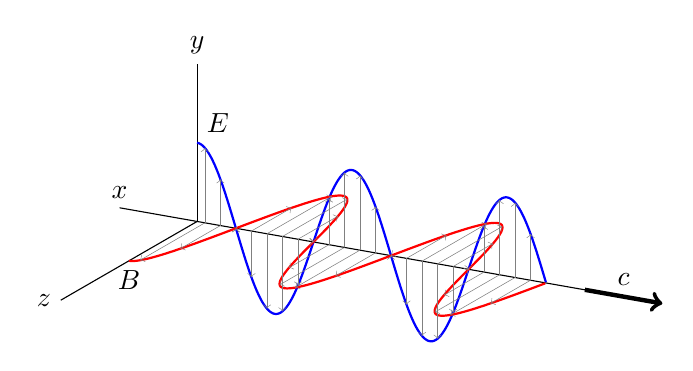
\begin{tikzpicture}[x={(-10:1cm)},y={(90:1cm)},z={(210:1cm)}]
    % Axes
    \draw (-1,0,0) node[above] {$x$} -- (5,0,0);
    \draw (0,0,0) -- (0,2,0) node[above] {$y$};
    \draw (0,0,0) -- (0,0,2) node[left] {$z$};
    % Propagation
    \draw[->,ultra thick] (5,0,0) -- node[above] {$c$} (6,0,0);
    % Waves
    \draw[blue,thick] plot[domain=0:4.5,samples=200] (\x,{cos(deg(pi*\x))},0);
    \draw[red,thick] plot[domain=0:4.5,samples=200] (\x,0,{cos(deg(pi*\x))});
    % Arrows
    \foreach \x in {0.1,0.3,...,4.4} {
      \draw[->,help lines] (\x,0,0) -- (\x,{cos(deg(pi*\x))},0);
      \draw[->,help lines] (\x,0,0) -- (\x,0,{cos(deg(pi*\x))});
    }
    % Labels
    \node[above right] at (0,1,0) {$\bm{E}$};
    \node[below] at (0,0,1) {$\bm{B}$};
    \end{tikzpicture}
    \captionsetup{type=figure,margin=1in,font=scriptsize}
    \captionof{figure}{An electromagnetic wave. The electric field is shown in blue; the magnetic field, in red. The electric and magnetic fields propagate in phase and perpendicular to each other.}
    \label{oQgjrD}
\end{center}

Let's recall the following definitions from the previous unit:

\begin{itemize}
\setlength\itemsep{-0.5ex}
    \item Wavelength is the distance between two wave crests or troughs, express in units of meters
    \item Frequency is the number of wave crests that pass a point per second, expressed in hertz (Hz)
    \item Amplitude is the height of the crest above the equilibrium line, or null point.
\end{itemize}

As mentioned, electromagnetic radiation takes several forms. These forms are characterized by a range of frequencies. Because frequency is inversely proportional to wavelength, any form of EMR can also be represented by its range of wavelengths. Figure \ref{TBWcbi} is the electromagnetic spectrum, which shows the frequency and wavelength ranges of various types of electromagnetic radiation.

\begin{center}
% \pgfplotsset{width=14cm, height=7cm}
\begin{tikzpicture}%[width=14cm,height=7cm]
    \begin{axis}[width=16cm, height=7cm,
        xlabel={Wavelength (m)},
        xticklabel style = {font=\tiny,yshift=0.2ex},
        xmin=10^-11,
        xmax=10^3,
        % x unit=\si{\micro\meter},
        xmode=log,
        ymin=0,ymax=1,
        height=3cm,
        yticklabels={},
        ytick=\empty,
        %legend cell align=left,
        %legend style={at={(1.19,1.5)},anchor=north}, %legend style={at={(0.85,-0.77)},anchor=north},
        x dir=reverse,
        ]
        \addplot[draw=none, name path=start, forget plot] coordinates{(10^-11,0)(10^-11,1)};
        \addplot[draw=none, name path=gamma, forget plot] coordinates{(10^-9,0)(10^-9,1)};
        \addplot[draw=none, name path=xrays, forget plot] coordinates{(10^-8,0)(10^-8,1)};
        \addplot[draw=none, name path=uv, forget plot] coordinates{(0.4*10^-6,0)(0.4*10^-6,1)};
        \addplot[draw=none, name path=visible, forget plot] coordinates{(0.7*10^-6,0)(0.7*10^-6,1)};
        \addplot[draw=none, name path=ir, forget plot] coordinates{(10^-3.5,0)(10^-3.5,1)};
        \addplot[draw=none, name path=microwave, forget plot] coordinates{(10^-1,0)(10^-1,1)};
        \addplot[draw=none, name path=radiowave, forget plot] coordinates{(10^3,0)(10^3,1)};

        \addplot[black!80, area legend] fill between[of=microwave and radiowave];
        \node[white] at (10,0.5) {Radio};
        \addplot[black!50, area legend] fill between[of=ir and microwave];
        \node[white] at (10^-2.3,0.5) {Microwave};
        \addplot[black!20, area legend] fill between[of=visible and ir];
        \node at (10^-4.9,0.5) {Infrared};
        \addplot[shading=visiblelight, area legend] fill between[of=uv and visible];
        \addplot[black!20, area legend] fill between[of=xrays and uv];
        \node at (10^-7.2,0.5) {UV};
        \addplot[black!50, area legend,pattern] fill between[of=gamma and xrays];
        \node[white] at (10^-8.5,0.5) {X};
        \addplot[black!80, area legend] fill between[of=start and gamma];
        \node[white] at (10^-10,0.5) {Gamma};
    \end{axis}

    \begin{axis}[width=16cm, height=7cm,
        xlabel={Frequency (Hz)},
        xticklabel style = {font=\tiny,yshift=0.2ex},
        xmin=3*10^5,xmax=3*10^19,
        % x unit=Hz,
        xmode=log,
        ymin=0,ymax=1,
        height=3cm,
        yticklabels={},
        ytick=\empty,
        %legend cell align=left,
        axis y line = none,
        axis x line* = top,
        %x dir=reverse,
        ]
    \end{axis}
\end{tikzpicture}
\captionsetup{type=figure,margin=1in,font=scriptsize}
\captionof{figure}{The electromagnetic spectrum, showing the major categories of electromagnetic waves. The range of frequencies and wavelengths is remarkable. The dividing line between some categories is only approximate, as some regions may overlap. Human eyes can only see visible light; all other regions are invisible to us.}
\label{TBWcbi}
\end{center}

Figure \ref{TBWcbi} has many parts. The narrow band that is visible light extends from lower-frequency red light to higher-frequency violet light. Frequencies just below visible are called \textit{infrared} (below red), and those just above are \textit{ultraviolet} (beyond violet).

\vspace{1em}

Radio waves, which are used for media broadcasts of TV and radio signals, occupy frequencies lower than infrared (IR). The microwave radiation is the same radiation that is used in your microwave oven. What we feel as radiant heat on your skin is also a form of low-frequency EMR. The high-frequency radiation to the right of ultraviolet (UV) includes X-rays and gamma ($\gamma$) rays.

\vspace{1em}

All these electromagnetic waves are the same form of radiation. They can all travel across empty space, and they all travel at the speed of light in a vacuum. The basic difference between types of radiation is their differing frequencies. Each frequency has an associated wavelength. Frequency and wavelength are \textit{inversely} proportional: as frequency increases across the spectrum, wavelength decreases. Each frequency also has an associated energy. Frequency and energy are \textit{directly} proportional: as the frequency of a wave increases, the energy also increases. For example, because ultraviolet waves occupy a higher frequency range than do infrared waves, the former carry more energy than the latter.


\clearpage

\subsection*{\ref{SJFjXy} Exercises}

\begin{exercise}
    Which of the following words best answers the question \textit{What is light}?

\begin{mdframed}[backgroundcolor=black!10]
    \begin{center}
        \textbf{
        acceleration \hfill
        charge \hfill
        current \hfill
        energy \hfill
        force \hfill
        momentum \hfill
        position \hfill
        velocity \hfill
        }
    \end{center}
\end{mdframed}
\end{exercise}

\begin{exercise}
    Physicists have divided the electromagnetic spectrum into how many different regions?
\end{exercise}

\begin{exercise}
    Name all the regions of the electromagnetic spectrum.
\end{exercise}

\begin{exercise}
    What is the basic difference between the various types of electromagnetic radiation?
\end{exercise}

\begin{exercise}
    How does wavelength change as frequency \textit{increases} across the electromagnetic spectrum?
\end{exercise}

\begin{exercise}
    Can electromagnetic waves travel through empty space (that is, through a vacuum)?
\end{exercise}

\begin{exercise}
    Create a table with the first column labeled ``visible'' and the second one ``invisible.'' Sort all regions of the electromagnetic spectrum into this table according to whether waves in those regions are visible or invisible to the human eye.
\end{exercise}


\begin{exercise}
    An electromagnetic wave consists of two oscillating fields that are perpendicular and in phase with each other. What are the names of each field?
\end{exercise}

\begin{exercise}
    Generate a radio wave by wiggling an electron. Access the \texttt[red]{PhET Simulation} ``Radio Waves \& Electromagnetic Fields'' (\href{https://phet.colorado.edu/en/simulations/radio-waves}{click here}). Click the play button in the center of the screen. Wiggle the electron, either in \texttt[red]{Manual} or \texttt[red]{Oscillate} mode. Observe how the oscillation of the electric charge results in the propagation in an electromagnetic wave. Use this simulation to explain, in your own words, how all electromagnetic radiation is generated.
\end{exercise}

\begin{exercise}
    The first wave below represents an electromagnetic wave in the X-ray region of the spectrum. If the second wave is not an X-ray, what type of electromagnetic radiation does it represent?
\end{exercise}

\begin{center}
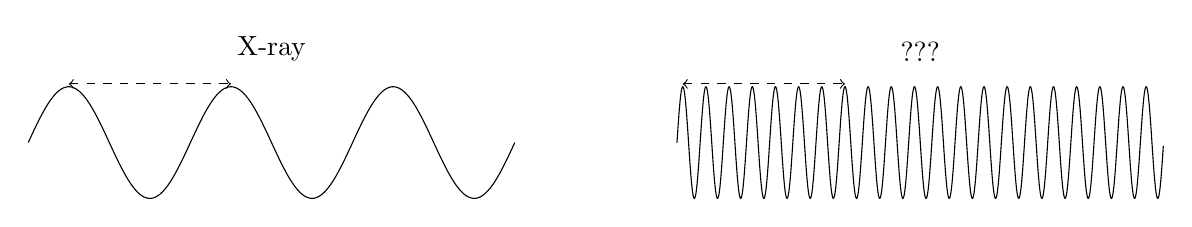
\begin{tikzpicture}
\begin{axis}[width=16cm,height=3cm,
    xmin=0,xmax=14,
    ymin=-1,ymax=1,
    clip=false,
    ticks=none,
    axis line style={draw=none}
    ]
    \draw[dashed,<->] (0.5,1.05) -- ++(axis direction cs: 2,0);
    \draw plot[domain=0:6*pi, samples=200] (\x/pi,{sin(\x r)});
    \node[above=2mm] at (3,1) {X-ray};
    \begin{scope}[shift={(axis direction cs: 8,0)}]
        \draw plot[domain=0:6*pi, samples=1000] (\x/pi,{sin(7/1*\x r)});
        \draw[dashed,<->] (0.5*1/7,1.05) -- ++(axis direction cs: 2,0);
        \node[above=2mm] at (3,1) {???};    
    \end{scope}
\end{axis}
\end{tikzpicture}
\end{center}

\begin{exercise}
    The first wave represents a microwave. If the second wave is an a different region of the spectrum, what type of electromagnetic wave is it?
\end{exercise}

\begin{center}
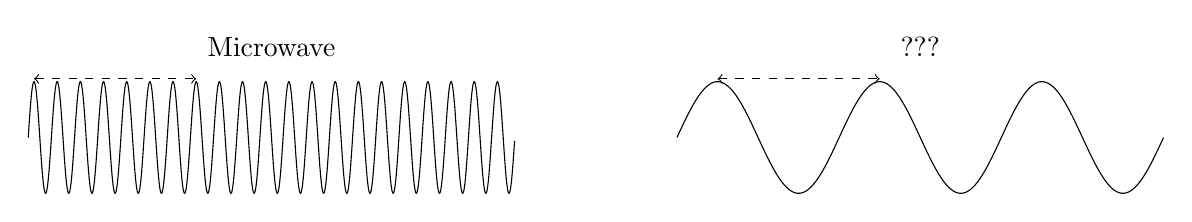
\begin{tikzpicture}
\begin{axis}[width=16cm,height=3cm,
    xmin=0,xmax=14,
    ymin=-1,ymax=1,
    clip=false,
    ticks=none,
    axis line style={draw=none}
    ]
    \draw plot[domain=0:6*pi, samples=1000] (\x/pi,{sin(7/1*\x r)});
    \draw[dashed,<->] (0.5*1/7,1.05) -- ++(axis direction cs: 2,0);
    \node[above=2mm] at (3,1) {Microwave};
    \begin{scope}[shift={(axis direction cs: 8,0)}]
        \draw plot[domain=0:6*pi, samples=200] (\x/pi,{sin(\x r)});
        \draw[dashed,<->] (0.5,1.05) -- ++(axis direction cs: 2,0);
        \node[above=2mm] at (3,1) {???};    
    \end{scope}
\end{axis}
\end{tikzpicture}
\end{center}


\clearpage

% \begin{figure}[h!]
%     \centering
%     \includegraphics[width=\textwidth]{figures/Ch15_Fig_EMSpectrum.png}
%     \caption*{The Electromagnetic Spectrum. Frequency ($f$) and wavelength ($\lambda$) relate to the speed of light ($c$) as $c = f \lambda$.}
% \end{figure}


\subsection{Visible Light} \label{pELT9m}

Visible light is the only region of the electromagnetic spectrum that is perceivable by human eyes. Wavelengths of visible light range from about \SI{380}{nm} (violet) to \SI{750}{nm} (red). The frequencies corresponding to these wavelengths are \SI{4.0e14}{Hz} at the red end to \SI{7.9e14}{Hz} at the violet end. This is a very narrow range, since the EM spectrum spans about 20 orders of magnitude.

\begin{center}
\begin{tikzpicture}
    \begin{axis}[width=14cm, height=7cm,
        xlabel={Wavelength (nm)}, 
        xtick={200,300,...,900},
        ymin=0,ymax=1,
        height=3cm,
        xmin=200,xmax=900,
        yticklabels={},
        ytick=\empty,
        axis lines=left,
        separate axis lines,
        y axis line style=white,
        x dir=reverse,
        clip=false,
        ]
        \addplot[draw=none, name path=uv, forget plot] coordinates{(360,0)(360,1)};
        \addplot[draw=none, name path=visible, forget plot] coordinates{(740,0)(740,1)};
        \addplot[shading=visiblelight, area legend] fill between[of=uv and visible];
        \node[align=center] at (800,0.5) {Infrared\\ (invisible)};
        \node[align=center] at (290,0.5) {Ultraviolet\\(invisible)};
        \node[above] at (550,1) {Visible light};
    \end{axis}
\end{tikzpicture}
\captionsetup{type=figure,margin=1in,font=scriptsize}
\captionof{figure}{A small part of the electromagnetic spectrum that includes its visible components. The divisions between infrared, visible, and ultraviolet are not perfectly distinct, nor are the divisions between the seven colors of the rainbow.}
\label{lyOjge}
\end{center}



% \begin{figure}[h!]
%     \centering
%     \includegraphics{figures/Unit12_Fig15.5.jpg}
%     \caption{The visible light portion of the electromagnetic spectrum.}
%     \label{fig:Unit12_Fig15.5}
% \end{figure}


Wavelengths of visible light are often given in nanometers (nm), so its useful to know how to convert nanometers to meters. One nanometer is one billionth of a meter (m):
\begin{equation} \label{LLLSU7}
    \SI{1}{nm} = \SI{1}{nanometer} = \SI{1e-9}{m}
\end{equation}

\begin{example}
    Yellow light has a wavelength of about \SI{600}{nm}. Convert this wavelength to meters.
\end{example}

\Solution Using Equation \eqref{LLLSU7}, 600 nanometers is converted to meters as

\begin{equation*}
    \SI{600}{\cancel\nano\meter} \times \frac{\SI{1e-9}{m}}{\SI{1}{\cancel\nano\meter}} = \SI{600e-9}{m} = \SI{6.00e-7}{m}
\end{equation*}

\solutionEnd

\vspace{1ex}

As seen in Figure \ref{lyOjge}, seven colors of the visible spectrum, in order of increasing frequency, are:

\begin{mdframed}[backgroundcolor=black!10]
\begin{center}
    \textbf{\hspace{5mm}
    red \hfill
    orange \hfill
    yellow \hfill
    green \hfill
    blue \hfill 
    indigo \hfill 
    violet \hspace{3mm} \hfill}
\end{center}
\end{mdframed}

To help you remember this order of the rainbow, you can remember the name \href{https://youtu.be/Gf33ueRXMzQ}{Roy G.~Biv}.

\vspace{1em}

How is it that human vision is confined to a tiny sliver of the whole electromagnetic spectrum? Color is detected by cells in the eye called \textit{cones}. Humans have three cones that are sensitive to three different ranges of electromagnetic wavelengths. They are called red, blue, and green cones, although these colors do not correspond exactly to the centers of the three ranges. The ranges of wavelengths that each cone detects are red, 500 to \SI{700}{nm}; green, 450 to \SI{630}{nm}; and blue, 400 to \SI{500}{nm}. Most primates also have three cones, while most non-primate mammals only have two. However, many birds, reptiles, amphibians, and insects have four or five different cones in their eyes. Some animals, like bees, see in ultraviolet, while rattlesnakes can see infrared light!

\vspace{1em}

Visible light also plays a major role in the ecological environment. Nearly all of our food depends on the photosynthesis process in plants. The energy for this process comes from the Sun in visible part of the spectrum. Without photosynthesis, we would also have almost no oxygen in the atmosphere.

\subsection*{\ref{pELT9m} Exercises}

\begin{exercise}
    Explain Roy G.~Biv.
\end{exercise}

\begin{exercise}
    Identify the name of the cells in your eyes that allow you to perceive color.
\end{exercise}

\begin{exercise}
    What are the seven colors of the rainbow in order of increasing \textit{wavelength}?
\end{exercise}

\begin{exercise}
    Between red and violet, which color represents the high-frequency limit of the visible spectrum?
\end{exercise}

\begin{exercise}
    Which color represents the long-wavelength limit of the visible spectrum?
\end{exercise}

\begin{exercise}
    Which region of the electromagnetic spectrum, apart from visible light, can bees see?
\end{exercise}

\begin{exercise}
    Which animal can see infrared light?
\end{exercise}

\begin{exercise} \label{lwLSKO}
    Sort the colors yellow, blue, and red from shortest wavelength to longest.
\end{exercise}

\begin{exercise}
    The first wave below represents the electromagnetic wave associated with the color cyan, also known as aqua blue. The second wave represents a different color of the visible light spectrum. Which colors can you rule \textit{out} to be represented by the second wave? Assume that the dashed double arrows are the same length and that cyan lies between green and blue.
\end{exercise}

\begin{center}
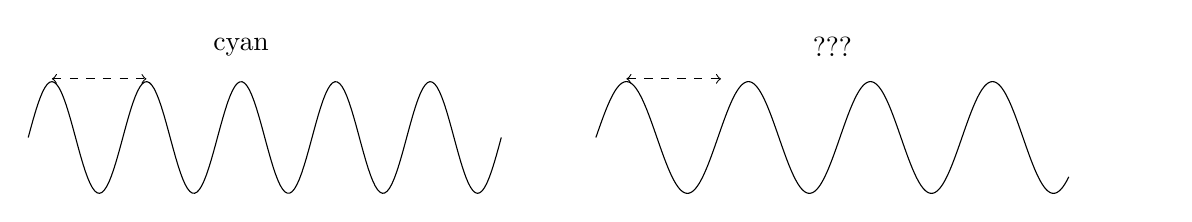
\begin{tikzpicture}
\begin{axis}[width=16cm,height=3cm,
    xmin=0,xmax=24,
    ymin=-1,ymax=1,
    clip=false,
    ticks=none,
    axis line style={draw=none}
    ]
    \draw[dashed,<->] (0.5,1.05) -- ++(axis direction cs: 2,0);
    \draw plot[domain=0:10*pi, samples=200] (\x/pi,{sin(\x r)});
    \node[above=2mm] at (4.5,1) {cyan};
    \begin{scope}[shift={(axis direction cs: 12,0)}]
        \draw[dashed,<->] (0.5*632/490,1.05) -- ++(axis direction cs: 2,0);
        \draw plot[domain=0:10*pi, samples=500] (\x/pi,{sin(490/632*\x r)});
        \node[above=2mm] at (5,1) {???};    
    \end{scope}
\end{axis}
\end{tikzpicture}

\vspace{1em}

\begin{tikzpicture}
    \begin{axis}[width=14cm, height=7cm,
        ymin=0,ymax=1,
        height=3cm,
        xmin=360,xmax=740,
        yticklabels={},
        ytick=\empty,
        axis lines=left,
        separate axis lines,
        y axis line style=white,
        x dir=reverse,
        clip=false,
        ticks=none,
        axis line style={draw=none}
        ]
        \addplot[draw=none, name path=uv, forget plot] coordinates{(360,0)(360,0.5)};
        \addplot[draw=none, name path=visible, forget plot] coordinates{(740,0)(740,0.5)};
        \addplot[shading=visiblelight, area legend] fill between[of=uv and visible];
        \draw[<-,thick] (490,0.5) -- ++(axis direction cs: 0,0.4) node[above] {cyan};
    \end{axis}
\end{tikzpicture}
\end{center}

\begin{exercise}
    Convert \SI{5798}{nm} to meters, writing in scientific notation.
\end{exercise}

\begin{exercise}
    Sort the colors in Exercises \ref{lwLSKO} from lowest frequency to highest.
\end{exercise}

\begin{exercise}
    What is the wavelength of a red light wave that has a frequency of \SI{4.746e14}{\Hz} if the wave travels through empty space at a speed of \SI{3.0e8}{m/s}? Express your answer in nanometers (nm).
\end{exercise}

\begin{exercise}
The Bacillus is a species of rod-shaped bacteria that are very common in nature. As shown below, a typical length is about 2 to 6 microns. Consider a green light wave, which has a wavelength of about 500 nanometers. About how many wave cycles of green light could fit along the length of the Bacillus below?
\end{exercise}


\begin{center}
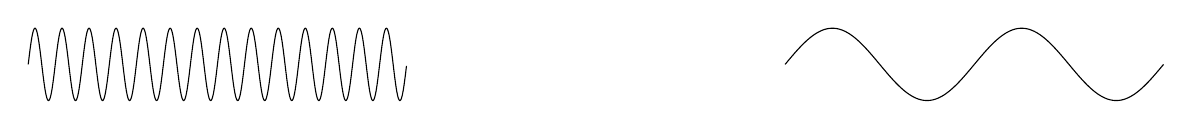
\begin{tikzpicture}
\begin{axis}[width=16cm,height=2.5cm,
    xmin=0,xmax=12,
    ymin=-1,ymax=1,
    clip=false,
    ticks=none,
    axis line style={draw=none}
    ]
    \draw plot[domain=0:4*pi, samples=1000] (\x/pi,{sin(7/1*\x r)});
    \begin{scope}[shift={(axis direction cs: 8,0)}]
        \draw plot[domain=0:4*pi, samples=200] (\x/pi,{sin(\x r)});   
    \end{scope}
\end{axis}
\end{tikzpicture}

\vspace{-1.5cm}

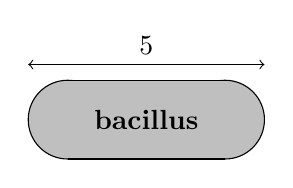
\begin{tikzpicture}
    \draw[fill=lightgray] (0,0) circle (0.5);
    \begin{scope}[shift={(2,0)}]
        \draw[fill=lightgray] (0,0) circle (0.5); 
    \end{scope}
    \fill[lightgray] (0,-0.5) rectangle ++(2,1) node[black,pos=0.5] {\textbf{bacillus}};
    \draw (0,0.5) -- ++(2,0)
          (0,-0.5) -- ++(2,0);
    \draw[<->] (-0.5,0.7) -- ++(3,0) node[above,pos=0.5] {\SI{5}{\micro\meter}};
\end{tikzpicture}
\end{center}









% \begin{figure}[h!]
%     \centering
%     \includegraphics[width=3in,trim={3in 2in 3.5in 2in},clip]{figures/Unit12_Fig_CampFire.jpg}
%     \caption{}
%     \label{fig:Unit12_Fig_CampFire}
% \end{figure}


\clearpage
\subsection{Low-Frequency Light} \label{8Wb3QO}

We define low-frequency light as electromagnetic waves with frequencies below visible light. The lower the frequency of an EM wave, the longer its wavelength and the lower its energy. Exposure to frequencies below visible light is generally safe. 

\vspace{1em}

Infrared is the region right below visible light. Wavelengths of infrared radiation span from about 750 nanometers to about 1 millimeter (mm). Although the human eye cannot see infrared radiation, the body can sense it. We feel it as heat or warmth, such as when we stand close to a campfire. Infrared waves have applications in heating, thermal imaging cameras heating, and lasers used in treating \href{https://www.tandfonline.com/doi/full/10.1080/13102818.2018.1544034}{gum disease}. 

\vspace{1em}

Microwaves have lower frequencies than infrared waves, through not as low as radio waves. The most famous application of microwaves is in your (aptly named) microwave oven. This oven cooks or warms food by irradiating it with EM radiation in the microwave frequency range. Most kitchen microwaves use a frequency of \SI{2.45e9}{Hz}. EM waves at this particular frequency have the right amount of energy to cause polar molecules\footnote{Polar molecules are those that have a partial charge separation.}, such as water, to rotate faster. The rotational energy of these molecules is given up to surrounding matter as heat. The end result: your food gets hot.

\vspace{1em}

Another application of microwaves is radar. Radar uses radiation with wavelengths similar to those of microwaves to detect the location and speed of distant objects, such as airplanes, weather formations, and motor vehicles. Radar information is obtained by receiving and analyzing the echoes of microwaves reflected by an object. The speed of the object can be measured using the Doppler shift of the returning waves. Astronomers use this same Doppler effect to measure the speed at which distant galaxies are moving away from us. In fact, in the 1960s, astronomers used these electromagnetic waves to prove that Mercury and Venus rotate and to measure these planets' rotation rates.

\vspace{1em}

Radio waves have the lowest frequencies---and, therefore, longest wavelengths---of the electromagnetic spectrum. Television, radio, cell phone, and remote-control devices all broadcast and/or receive signals with in radio wavelengths. One medical-imaging technique is magnetic resonance imaging (MRI). MRI is an important imaging and research tool in medicine, producing highly detailed two- and three-dimensional images. Radio waves are broadcast, absorbed, and re-emitted in a resonance process that is sensitive to the density of nuclei, usually hydrogen nuclei---protons.

\clearpage
\subsection*{\ref{8Wb3QO} Exercises}

% \begin{exercise}
%     Watch ``Shirtless Heat Loss Experiment in Freezing Conditions'' by \texttt{BBC Earth Unplugged} on \texttt{YouTube} (\href{https://youtu.be/o2bzGyc6WAg}{click here}) for a visual of infrared radiation. Since infrared radiation is invisible to human eyes, what does the red color in the video represent? What does blue represent?
% \end{exercise}

\begin{exercise} \label{wqaTm6}
    When water molecules are bathed in electromagnetic radiation at just the right frequency, they get begin to vibrate and give off heat to their environment. What frequency must these waves have for this phenomenon to occur? Write the number in scientific and decimal notation.
\end{exercise}

\begin{exercise}
    To what region of the electromagnetic spectrum do the waves from Exercise \ref{wqaTm6} belong? 
\end{exercise}

\begin{exercise}
    What happens to the energy of electromagnetic radiation as frequency decreases?
\end{exercise}

\begin{exercise}
    How do humans detect infrared radiation?
\end{exercise}

\begin{exercise}
    Explain some applications of microwaves in astronomy. 
\end{exercise}

\begin{exercise}
    Which type of electromagnetic wave has the longest wavelength of the whole spectrum?
\end{exercise}

\begin{exercise}
    In what medical technology are radio waves used?
\end{exercise}

\clearpage
\subsection{High-Frequency Light} \label{QoTj3l}

We define high-frequency light as electromagnetic waves with frequencies above visible light. Exposure to any radiation with frequencies greater than those of visible light carries some health hazards. All types of radiation in this range are known to cause cell damage. The danger is related to the high energy and penetrating ability of these EM waves. The likelihood of being harmed by any of this radiation depends largely on the amount of exposure. 



\vspace{1em}

Ultraviolet (UV) radiation comes after visible light on the electromagnetic spectrum.  Since \textit{ultra} means extreme or beyond, this region has higher frequencies than violet color. A major source of UV light on Earth is the Sun, though many high-frequency UV rays get absorbed by the atmosphere before they reach the ground. Most people try to reduce exposure to UV radiation from sunlight by using sunscreen and protective clothing. Ultraviolet light has a variety of useful applications. For example, black-lights are used by detectives to see bodily fluids. Also, UV lights may be installed inside air ducts on AC units to kill bacteria on surfaces.  

\vspace{1em}

X-rays have higher frequencies than ultraviolet waves. This type of electromagnetic radiation is widely known for its application in the medical field. Doctors and dentists use X-rays to diagnose medical problems, but the intensity of the radiation used is extremely low and therefore safe. While pregnant women should not be exposed to X-rays, even at low doses, some babies get chest X-rays a few months after birth. Medical X-ray images are possible because of the absorption of X-rays by electrons. Calcium atoms, which are plentiful in teeth and bones, carry lot of electrons for X-ray absorption, more so than carbon, oxygen, and other organic atoms. That's why teeth and bones make excellent X-ray images.

\vspace{1em}

Gamma rays have the highest frequencies of the entire electromagnetic spectrum. Due to their high frequencies, they have the highest energies of all EM waves. In 1986, the core of the Chernobyl nuclear reactor at Pripyat in present-day Ukraine exploded. This disaster was caused by human error and serious flaws in the design of the reactor. The exposed core released enormous amounts of deadly gamma ray radiation. Workers and firefighters who got too close to the open core---several dozen meters away---died from radiation poisoning days or weeks after exposure. To this day, Pripyat is an abandoned city due to the lingering presence of gamma rays. But aside from this rare catastrophe, gamma rays are rarely observed on Earth. While they are generated in tiny amounts during a lighting strike, most gamma rays are generated in high-energy events in distant parts of outer space. 

\subsection*{\ref{QoTj3l} Exercises}

\begin{exercise}
    Which type of electromagnetic radiation has the shortest wavelengths?
\end{exercise}

\begin{exercise}
    Which form of EM radiation has the most penetrating ability?
\end{exercise}

\begin{exercise}
    Why are high-frequency gamma rays more dangerous to humans than visible light?
\end{exercise}



\subsection{The Speed of Light} \label{VDAtHN}

A vacuum is a region of space that is devoid of all matter. For this reason, a vacuum is also known as ``empty space.'' Electromagnetic waves, unlike sound waves or mechanical waves, \textit{can} travel through a vacuum. EM waves travel through empty space, and they also travel through some media, like air, glass, and water. But electromagnetic waves travel fastest through a vacuum, at a rate known as the speed of light:

\begin{equation}
    c = \SI{3.0e8}{m/s}
\end{equation}

The speed of light is the upper limit of speed in the universe, since nothing can travel faster than light.

In a vacuum, all electromagnetic radiation travels at a speed of \SI{3.0e8}{m/s} (671 million miles per hour), which is known as the ``speed of light'' and is given the symbol

\begin{equation*}
    c = \SI{3.0e8}{m/s}
\end{equation*}

When light travels through a physical medium, its speed is always less than the speed of light ($c$).

\subsection*{\ref{VDAtHN} Exercises}

\begin{exercise}
    True or false? Light requires a medium to propagate.
\end{exercise}

\begin{exercise}
    What is the value of $c$, the speed of light in a vacuum?
\end{exercise}

\begin{exercise}
    Saturn is \SI{1.43e12}{m} from the Sun. How many minutes does it take the Sun’s light to reach Saturn? To get full credit, show all your work.
\end{exercise}

\clearpage
\subsection*{References}

\begin{itemize}
\setlength\itemsep{0.1ex}
    \item \texttt{YouTube}: ``What Is a Field?'' by \texttt{Scientific American} (\href{https://youtu.be/7BK166SL-ig}{click here}). A field is like a fluid that fills all space. Waves can propagate through that fluid.
    \item \texttt{YouTube}: ``They Might Be Giants -- Roy G.~Biv'' by \texttt{TMBGkids} (\href{https://youtu.be/Gf33ueRXMzQ}{click here})
    \item \texttt{PhET Simulation}: ``Waves Intro'' (\href{https://phet.colorado.edu/sims/html/waves-intro/latest/waves-intro_en.html}{click here}). Open the \texttt{Light} panel. Check \texttt{Graph} and click the green button on the laser to see disturbances in the electric field.
    \item \texttt{PhET Simulation}: Radio Waves \& Electromagnetic Fields (\href{https://phet.colorado.edu/sims/cheerpj/radio-waves/latest/radio-waves.html?simulation=radio-waves}{click here})
    \item \href{https://science.nasa.gov/ems/01_intro}{NASA: Introduction to the Electromagnetic Spectrum}
    \item \texttt{YouTube}: ``Light waves, visible and invisible - Lucianne Walkowicz'' by \texttt{TED-Ed} (\href{https://youtu.be/O0PawPSdk28}{click here})
    \item \texttt{YouTube}: ``The Electromagnetic Spectrum'' by \texttt{Best0fScience} (\href{https://youtu.be/cfXzwh3KadE}{click here})
    \item \texttt{YouTube}: ``Shirtless Heat Loss Experiment in Freezing Conditions'' by \texttt{BBC Earth Unplugged} (\href{https://youtu.be/o2bzGyc6WAg}{click here})
    \item \href{https://youtu.be/QALt_ja2HGY}{UV Light as Fast as Possible}
    \item \href{https://youtu.be/gsV7SJDDCY4}{How X-rays see through your skin}
    \item \textit{Cosmos}, Episode 4, minute 31:20 for using X-rays to ``see'' black holes.
    \item \texttt{OpenStax} (\href{https://openstax.org/books/physics/pages/15-1-the-electromagnetic-spectrum#Table_15_01}{click here}). Electromagnetic waves. This table shows how each type of electromagnetic (EM) radiation is produced, how it is applied, as well as environmental and health issues associated with it.
    \item \textit{Cosmos}: ``Hiding in the Light'' (Sn.~1, Ep.~5). Light dispersed through a prism (28:31 -- 29:31); sunlight, color, wave energy, rods and cones (30:50 -- 33:06); spectral lines and quantum mechanics (33:10); symphony of electromagnetic radiation (41:40 -- 43:18)
\end{itemize}

\clearpage
\printnoidxglossaries


\end{document}






